\documentclass[11pt,letterpaper]{article}


% pmml  arff  openannotation

\usepackage[T1]{fontenc}
\usepackage{tgtermes}

\usepackage[hang,flushmargin]{footmisc}

\usepackage{titlesec}

\titlespacing*{\section}
{0pt}{4.5ex plus 1ex minus .5ex}{.9ex plus .2ex}

%\usepackage{mathptmx}

\usepackage{eso-pic}

%\setlength\parindent{0pt}

\AddToShipoutPictureBG{%

\ifnum\value{page}>1{
\AtTextUpperLeft{
\makebox[20.5cm][r]{
\raisebox{-1.95cm}{%
{\transparent{0.3}{
\includegraphics[width=0.29\textwidth]{e-logo.png}}	}} } }
}\fi
}

\AddToShipoutPicture{%
{
 {\color{blGreen!70!red}\transparent{0.9}{\put(0,0){\rule{3pt}{\paperheight}}}}%
 {\color{darkRed!70!purple}\transparent{1}\put(3,0){{\rule{4pt}{\paperheight}}}}
% {\color{logoPeach!80!cyan}\transparent{0.5}{\put(0,700){\rule{1cm}{.6cm}}}}%
% {\color{darkRed!60!cyan}\transparent{0.7}\put(0,706){{\rule{1cm}{.6cm}}}}
% \put(18,726){\thepage}
% \transparent{0.8}
}
}

\AddToShipoutPicture{%
\ifnum\value{page}=1
\put(257.5,998){%
	\transparent{0.7}{
		
\includegraphics[width=0.2\textwidth]{logo.png}}}
\fi
}	



\AddToShipoutPicture{%
\ifnum\value{page}>1
{\color{blGreen!70!red}\transparent{0.9}{\put(300,8){\rule{0.5\paperwidth}{.3cm}}}}%
{\color{inOne}\transparent{0.8}{\put(300,10){\rule{0.5\paperwidth}{.3cm}}}}%
{\color{inTwo}\transparent{0.3}\put(300,13){{\rule{0.5\paperwidth}{.3cm}}}}

\put(301,16){%
\transparent{0.7}{

\includegraphics[width=0.2\textwidth]{logo.png}} }

{\color{blGreen!70!red}\transparent{0.9}{\put(5.6,5){\rule{0.5\paperwidth}{.4cm}}}}%
{\color{inOne}\transparent{1}{\put(5.6,10){\rule{0.5\paperwidth}{.4cm}}}}%
{\color{inTwo}\transparent{0.3}\put(5.6,15){{\rule{0.5\paperwidth}{.4cm}}}}

\fi
}

%\pagestyle{empty} % no page number
%\parskip 7.2pt    % space between paragraphs
%\parindent 12pt   % indent for new paragraph
%\textwidth 4.5in  % width of text
%\columnsep 0.8in  % separation between columns

%\setlength{\footskip}{7pt}

\usepackage[paperheight=15in,paperwidth=8.5in]{geometry}
\geometry{left=.65in,top=.65in,right=.45in,bottom=1.25in} %margins

\renewcommand{\thepage}{\raisebox{-4pt}{\arabic{page}}}

\renewcommand{\footnoterule}{%
	\kern -3pt
	\hrule width .92\textwidth height .5pt
	\kern 10pt
}


\usepackage[hyphens]{url}
\newcommand{\biburl}[1]{ {\fontfamily{gar}\selectfont{\textcolor[rgb]{.2,.6,0}%
{\scriptsize {\url{#1}}}}}}

%\linespread{1.3}

\newcommand{\sectsp}{\vspace{12pt}}

\usepackage{graphicx}
\usepackage{color,framed}

\usepackage{textcomp}

\usepackage{float}

\usepackage{mdframed}


\usepackage{setspace}
\newcommand{\rpdfNotice}[1]{\begin{onehalfspacing}{

\Large #1

}\end{onehalfspacing}}

\usepackage{xcolor}

\usepackage[hyphenbreaks]{breakurl}
\usepackage[hyphens]{url}

\usepackage{hyperref}
\newcommand{\rpdfLink}[1]{\href{#1}{\small{#1}}}
\newcommand{\dblHref}[1]{\href{#1}{\small{\burl{#1}}}}
\newcommand{\browseHref}[2]{\href{#1}{\Large #2}}

\colorlet{blCyan}{cyan!50!blue}

\definecolor{darkRed}{rgb}{.2,.0,.1}


\definecolor{blGreen}{rgb}{.2,.7,.3}

\definecolor{darkBlGreen}{rgb}{.1,.3,.2}

\definecolor{oldBlColor}{rgb}{.2,.7,.3}

\definecolor{blColor}{rgb}{.1,.3,.2}

\definecolor{elColor}{rgb}{.2,.1,0}
\definecolor{flColor}{rgb}{0.7,0.3,0.3}

\definecolor{logoOrange}{RGB}{108, 18, 30}
\definecolor{logoGreen}{RGB}{85, 153, 89}
\definecolor{logoPurple}{RGB}{200, 208, 30}

\definecolor{logoBlue}{RGB}{4, 2, 25}
\definecolor{logoPeach}{RGB}{255, 159, 102}
\definecolor{logoCyan}{RGB}{66, 206, 244}
\definecolor{logoRed}{rgb}{.3,0,0}

\newcommand{\colorq}[1]{{\color{logoOrange!70!black}{\q{\small\textbf{#1}}}}}

\definecolor{inOne}{rgb}{0.122, 0.435, 0.698}% Rule colour
\definecolor{inTwo}{rgb}{0.122, 0.698, 0.435}% Rule colour

\definecolor{outOne}{rgb}{0.435, 0.698, 0.122}% Rule colour
\definecolor{outTwo}{rgb}{0.698, 0.435, 0.122}% Rule colour

\usepackage[many]{tcolorbox}% http://ctan.org/pkg/tcolorbox

\usepackage{transparent}

\newlength{\bsep}
\setlength{\bsep}{-1pt}
\let\xbibitem\bibitem
\renewcommand{\bibitem}[2]{\vspace{\bsep}\xbibitem{#1}{#2}}

\newenvironment{cframed}{\begin{mdframed}[linecolor=logoPeach,linewidth=0.4mm]}{\end{mdframed}}

\newenvironment{ccframed}{\begin{mdframed}[backgroundcolor=logoGreen!5,linecolor=logoCyan!50!black,linewidth=0.4mm]}{\end{mdframed}}

\usepackage{aurical}
\usepackage[T1]{fontenc}

\usepackage{relsize}

\newcommand{\bref}[1]{\hspace*{1pt}\textbf{\ref{#1}}}

\newcommand{\pseudoIndent}{

\vspace{10pt}\hspace*{12pt}}

\newcommand{\YPDFI}{{\fontfamily{fvs}\selectfont YPDF-Interactive}}

%
\newcommand{\deconum}[1]{{\protect\raisebox{-1pt}{{\LARGE #1}}}}

\newcommand{\visavis}{vis-\`a-vis}

\newcommand{\VersatileUX}{{\color{red!85!black}{\Fontauri Versatile}}%
{{\fontfamily{qhv}\selectfont\smaller UX}}}

\newcommand{\NDPCloud}{{\color{red!15!black}%
{\fontfamily{qhv}\selectfont {\smaller NDP C{\smaller LOUD}}}}}

\newcommand{\MThreeK}{{\color{blGreen!45!black}%
{\fontfamily{qhv}\fontsize{10}{8}\selectfont {M3K}}}}


\newcommand{\lfNDPCloud}{{\color{red!15!black}%
{\fontfamily{qhv}\selectfont N{\smaller DP C{\smaller LOUD}}}}}

\newcommand{\textds}[1]{{\fontfamily{lmdh}\selectfont{%
\raisebox{-1pt}{#1}}}}

\newcommand{\dsC}{{\textds{ds}{\fontfamily{qhv}\selectfont \raisebox{-1pt}
{\color{red!15!black}{C}}}}}

\definecolor{tcolor}{RGB}{24,52,61}

\newcommand{\CCpp}{\resizebox{!}{7pt}{\AcronymText{C}}/\Cpp{}}
\newcommand{\NoSQL}{\resizebox{!}{7pt}{\AcronymText{NoSQL}}}
\newcommand{\SQL}{\resizebox{!}{7pt}{\AcronymText{SQL}}}

\newcommand{\NCBI}{\resizebox{!}{7pt}{\AcronymText{NCBI}}}

\newcommand{\HTXN}{\resizebox{!}{7pt}{\AcronymText{HTXN}}}

\newcommand{\TDM}{\resizebox{!}{7pt}{\AcronymText{TDM}}}

\newcommand{\lHTXN}{\resizebox{!}{7.5pt}{\AcronymText{HTXN}}}
\newcommand{\lsHTXN}{\resizebox{!}{9.5pt}{\AcronymText{\textcolor{tcolor}{HTXN}}}}

\newcommand{\LAF}{\resizebox{!}{7pt}{\AcronymText{LAF}}}

\newcommand{\UDpipe}{\resizebox{!}{7pt}{\AcronymText{UDpipe}}}

\newcommand{\C}{\resizebox{!}{7pt}{\AcronymText{C}}}


\usepackage{mdframed}

\newcommand{\cframedboxpanda}[1]{\begin{mdframed}[linecolor=yellow!70!blue,linewidth=0.4mm]#1\end{mdframed}}


\newcommand{\PVD}{\resizebox{!}{7pt}{\AcronymText{PVD}}}

\newcommand{\THQL}{\resizebox{!}{7pt}{\AcronymText{THQL}}}
\newcommand{\lTHQL}{\resizebox{!}{7.5pt}{\AcronymText{THQL}}}

\newcommand{\SDK}{\resizebox{!}{7pt}{\AcronymText{SDK}}}
\newcommand{\NLP}{\resizebox{!}{7pt}{\AcronymText{NLP}}}

\newcommand{\AXF}{\resizebox{!}{7pt}{\AcronymText{AXF}}}
\newcommand{\lAXF}{\resizebox{!}{7.5pt}{\AcronymText{AXF}}}
\newcommand{\lsAXF}{\resizebox{!}{8.5pt}{\AcronymText{AXF}}}

\newcommand{\AXFD}{\resizebox{!}{7pt}{\AcronymText{AXFD}}}
\newcommand{\lAXFD}{\resizebox{!}{7.5pt}{\AcronymText{AXFD}}}

\newcommand{\IJST}{\resizebox{!}{7pt}{\AcronymText{IJST}}}

\newcommand{\BioC}{\resizebox{!}{7pt}{\AcronymText{BioC}}}

\newcommand{\CoNLL}{\resizebox{!}{7pt}{\AcronymText{CoNLL}}}
\newcommand{\CoNLLU}{\resizebox{!}{7pt}{\AcronymText{CoNLL-U}}}

\newcommand{\sapp}{\resizebox{!}{7pt}{\AcronymText{Sapien+}}}
\newcommand{\lsapp}{\resizebox{!}{8.5pt}{\AcronymText{Sapien+}}}
\newcommand{\lssapp}{\resizebox{!}{9.5pt}{\AcronymText{Sapien+}}}

\newcommand{\ePub}{\resizebox{!}{7pt}{\AcronymText{ePub}}}

%\lsLPF


\newcommand{\GIT}{\resizebox{!}{7pt}{\AcronymText{GIT}}}

\newcommand{\LPF}{\resizebox{!}{7pt}{\AcronymText{LPF}}}
\newcommand{\lLPF}{\resizebox{!}{8.5pt}{\AcronymText{LPF}}}
\newcommand{\lsLPF}{\resizebox{!}{9.5pt}{\AcronymText{LPF}}}

\makeatletter

\newcommand*\getX[1]{\expandafter\getX@i#1\@nil}

\newcommand*\getY[1]{\expandafter\getY@i#1\@nil}
\def\getX@i#1,#2\@nil{#1}
\def\getY@i#1,#2\@nil{#2}
\makeatother
	
\newcommand{\rectann}[9]{%
\path [draw=#1,draw opacity=#2,line width=#3, fill=#4, fill opacity = #5, even odd rule] %
(#6) rectangle(\getX{#6}+#7,\getY{#6}+#8)
({\getX{#6}+((#7-(#7*#9))/2)},{\getY{#6}+((#8-(#8*#9))/2)}) rectangle %
({\getX{#6}+((#7-(#7*#9))/2)+#7*#9},{\getY{#6}+((#8-(#8*#9))/2)+#8*#9});}


\definecolor{pfcolor}{RGB}{94, 54, 73}

\newcommand{\EPF}{\resizebox{!}{7pt}{\AcronymText{ETS{\color{pfcolor}pf}}}}
\newcommand{\lEPF}{\resizebox{!}{8.5pt}{\AcronymText{ETS{\color{pfcolor}pf}}}}
\newcommand{\lsEPF}{\resizebox{!}{9.5pt}{\AcronymText{ETS{\color{pfcolor}pf}}}}


\newcommand{\XPDF}{\resizebox{!}{7pt}{\AcronymText{XPDF}}}

\newcommand{\GRE}{\resizebox{!}{8.5pt}{\AcronymText{GRE}}}

\newcommand{\lMOSAIC}{\resizebox{!}{8.5pt}{\AcronymText{MOSAIC}}}

\newcommand{\XML}{\resizebox{!}{7pt}{\AcronymText{XML}}}
\newcommand{\RDF}{\resizebox{!}{7pt}{\AcronymText{RDF}}}
\newcommand{\DOM}{\resizebox{!}{7pt}{\AcronymText{DOM}}}

\newcommand{\Covid}{\resizebox{!}{7pt}{\AcronymText{Covid-19}}}

\newcommand{\CLang}{\resizebox{!}{7pt}{\AcronymText{C}}}

\newcommand{\HNaN}{\resizebox{!}{7pt}{\AcronymText{HN%
\textsc{a}N}}}

\newcommand{\JSON}{\resizebox{!}{7pt}{\AcronymText{JSON}}}

\newcommand{\MeshLab}{\resizebox{!}{7pt}{\AcronymText{MeshLab}}}
\newcommand{\IQmol}{\resizebox{!}{7pt}{\AcronymText{IQmol}}}

\newcommand{\SGML}{\resizebox{!}{7pt}{\AcronymText{SGML}}}

\newcommand{\ASCII}{\resizebox{!}{7pt}{\AcronymText{ASCII}}}

\newcommand{\GUI}{\resizebox{!}{7pt}{\AcronymText{GUI}}}

\newcommand{\API}{\resizebox{!}{7pt}{\AcronymText{API}}}

\newcommand{\JATS}{\resizebox{!}{7pt}{\AcronymText{JATS}}}


\newcommand{\SDI}{\resizebox{!}{7pt}{\AcronymText{SDI}}}
\newcommand{\SDIV}{\resizebox{!}{7pt}{\AcronymText{SDIV}}}



\newcommand{\IDE}{\resizebox{!}{7pt}{\AcronymText{IDE}}}

\newcommand{\ThreeD}{\resizebox{!}{7pt}{\AcronymText{3D}}}

\newcommand{\FAIR}{\resizebox{!}{7pt}{\AcronymText{FAIR}}}

\newcommand{\QNetworkManager}{\resizebox{!}{7pt}{\AcronymText{QNetworkManager}}}
\newcommand{\QTextDocument}{\resizebox{!}{7pt}{\AcronymText{QTextDocument}}}
\newcommand{\QWebEngineView}{\resizebox{!}{7pt}{\AcronymText{QWebEngineView}}}
\newcommand{\HTTP}{\resizebox{!}{7pt}{\AcronymText{HTTP}}}


\newcommand{\lAcronymTextNC}[2]{{\fontfamily{fvs}\selectfont {\Large{#1}}{\large{#2}}}}

\newcommand{\AcronymTextNC}[1]{{\fontfamily{fvs}\selectfont {\large #1}}}


\colorlet{orr}{orange!60!red}

\newcommand{\textscc}[1]{{\color{orr!35!black}{{%
						\fontfamily{Cabin-TLF}\fontseries{b}\selectfont{\textsc{\scriptsize{#1}}}}}}}


\newcommand{\textsccserif}[1]{{\color{orr!35!black}{{%
				\scriptsize{\textbf{#1}}}}}}


\newcommand{\iXPDF}{\resizebox{!}{7pt}{\textsccserif{%
\textit{XPDF}}}}

\newcommand{\iEPF}{\resizebox{!}{7pt}{\textsccserif{%
\textit{ETSpf}}}}

\newcommand{\iSDI}{\resizebox{!}{7pt}{\textsccserif{%
\textit{SDI}}}}

\newcommand{\iHTXN}{\resizebox{!}{7pt}{\textsccserif{%
\textit{HTXN}}}}


\newcommand{\AcronymText}[1]{{\textscc{#1}}}

\newcommand{\AcronymTextser}[1]{{\textsccserif{#1}}}


\newcommand{\mAcronymText}[1]{{\textscc{\normalsize{#1}}}}

\newcommand{\FASTA}{{\resizebox{!}{7pt}{\AcronymText{FASTA}}}}
\newcommand{\SRA}{{\resizebox{!}{7pt}{\AcronymText{SRA}}}}
\newcommand{\DNA}{{\resizebox{!}{7pt}{\AcronymText{DNA}}}}
\newcommand{\MAP}{{\resizebox{!}{7pt}{\AcronymText{MAP}}}}
\newcommand{\EPS}{{\resizebox{!}{7pt}{\AcronymText{EPS}}}}
\newcommand{\CSV}{{\resizebox{!}{7pt}{\AcronymText{CSV}}}}
\newcommand{\PDB}{{\resizebox{!}{7pt}{\AcronymText{PDB}}}}

\newcommand{\TeXMECS}{\resizebox{!}{7pt}{\AcronymText{TeXMECS}}}

% pmml  arff  openannotation

\newcommand{\PMML}{\resizebox{!}{7pt}{\AcronymText{PMML}}}
\newcommand{\ARFF}{\resizebox{!}{7pt}{\AcronymText{ARFF}}}
\newcommand{\IeXML}{\resizebox{!}{7pt}{\AcronymText{IeXML}}}


\newcommand{\NGML}{\resizebox{!}{7pt}{\AcronymText{NGML}}}

\newcommand{\Cpp}{\resizebox{!}{7pt}{\AcronymText{C++}}}

\newcommand{\WhiteDB}{\resizebox{!}{7pt}{\AcronymText{WhiteDB}}}

\colorlet{drp}{darkRed!70!purple}

%\newcommand{\MOSAIC}{{\color{drp}{\AcronymTextNC{\scriptsize{MOSAIC}}}}}

\newcommand{\MOSAIC}{\resizebox{!}{7pt}{\AcronymText{MOSAIC}}}


\newcommand{\mMOSAIC}{{\color{drp}{\AcronymTextNC{\normalsize{MOSAIC}}}}}

\newcommand{\MOSAICVM}{\mMOSAIC-\mAcronymText{VM}}

\newcommand{\sMOSAICVM}{\resizebox{!}{7pt}{\MOSAICVM}}
\newcommand{\sMOSAIC}{\resizebox{!}{7pt}{\MOSAIC}}

\newcommand{\LDOM}{\resizebox{!}{7pt}{\AcronymText{LDOM}}}
\newcommand{\Cnineteen}{\resizebox{!}{7pt}{\AcronymText{CORD-19}}}

\newcommand{\lCnineteen}{\resizebox{!}{7.5pt}{\AcronymText{CORD-19}}}


\newcommand{\MOL}{\resizebox{!}{7pt}{\AcronymText{MOL}}}

\newcommand{\ACL}{\resizebox{!}{7pt}{\AcronymText{ACL}}}

\newcommand{\LXCR}{\resizebox{!}{7pt}{\AcronymText{LXCR}}}
\newcommand{\lLXCR}{\resizebox{!}{8.5pt}{\AcronymText{LXCR}}}
\newcommand{\lsLXCR}{\resizebox{!}{9.5pt}{\AcronymText{LXCR}}}

%\newcommand{\lMOSAIC}{{\color{drp}{\lAcronymTextNC{M}{OSAIC}}}}
\newcommand{\lfMOSAIC}{\resizebox{!}{9pt}{{\color{drp}{\lAcronymTextNC{M}{OSAIC}}}}}

\newcommand{\Mosaic}{\resizebox{!}{7pt}{\MOSAIC}}
\newcommand{\MosaicPortal}{{\color{drp}{\AcronymTextNC{MOSAIC Portal}}}}

\newcommand{\RnD}{\resizebox{!}{7pt}{\AcronymText{R\&D}}}
\newcommand{\QtCpp}{\resizebox{!}{8.5pt}{\AcronymText{Qt/C++}}}
\newcommand{\Qt}{\resizebox{!}{7pt}{\AcronymText{Qt}}}
\newcommand{\QtSQL}{\resizebox{!}{7pt}{\AcronymText{QtSQL}}}

\newcommand{\HTML}{\resizebox{!}{7pt}{\AcronymText{HTML}}}
\newcommand{\PDF}{\resizebox{!}{7pt}{\AcronymText{PDF}}}

\newcommand{\R}{\resizebox{!}{7pt}{\AcronymText{R}}}
\newcommand{\SciXML}{\resizebox{!}{7pt}{\AcronymText{SciXML}}}



\newcommand{\lGRE}{\resizebox{!}{7pt}{\AcronymText{GRE}}}

\newcommand{\p}[1]{

\vspace{.75em}#1}

\newcommand{\q}[1]{{\fontfamily{qcr}\selectfont ``}#1{\fontfamily{qcr}\selectfont ''}} 

%\newcommand{\deconum}[1]{{\textcircled{#1}}}


\renewcommand{\thesection}{\protect\mbox{\deconum{\Roman{section}}}}
\renewcommand{\thesubsection}{\arabic{section}.\arabic{subsection}}

\newcommand{\llMOSAIC}{\mbox{{\LARGE MOSAIC}}}
%\newcommand{\lfMOSAIC}{\mbox{M\small{OSAIC}}}

\newcommand{\llMosaic}{\llMOSAIC}
\newcommand{\lMosaic}{\lMOSAIC}
\newcommand{\lfMosaic}{\lfMOSAIC}


\newcommand{\llWC}{\mbox{{\LARGE WhiteCharmDB}}}

\newcommand{\llwh}{\mbox{{\LARGE White}}}
\newcommand{\llch}{\mbox{{\LARGE CharmDB}}}

\usepackage{enumitem}
%\usepackage{listings}

\colorlet{dsl}{purple!20!brown}
\colorlet{dslr}{dsl!50!blue}

\setlist[description]{%
  topsep=10pt,
  labelsep=12pt,
  itemsep=12pt,               % space between items
  %font={\bfseries\sffamily}, % set the label font
  font=\normalfont\bfseries\color{dslr!50!black}, % if colour is needed
}

\setlist[enumerate]{%
  topsep=3pt,               % space before start / after end of list
  itemsep=-2pt,               % space between items
  font={\bfseries\sffamily}, % set the label font
%  font={\bfseries\sffamily\color{red}}, % if colour is needed
}

%\usepackage{tcolorbox}

\newcommand{\slead}[1]{%
\noindent{\raisebox{2pt}{\relscale{1.15}{{{%
\fcolorbox{logoCyan!50!black}{logoGreen!5}{#1}
}}}}}\hspace{.5em}}


\let\OldLaTeX\LaTeX

\renewcommand{\LaTeX}{\resizebox{!}{7pt}{\color{orr!35!black}{\OldLaTeX}}}

\let\OldTeX\TeX

\renewcommand{\TeX}{\resizebox{!}{7pt}{\color{orr!35!black}{\OldTeX}}}


\newcommand{\LargeLaTeX}{\resizebox{!}{8.5pt}{\color{orr!35!black}{\OldLaTeX}}}

\setlength\parindent{0pt}
%\setlength\parindent{24pt}
%
\usepackage{titlesec}
\usepackage[hyphens]{url}

\newsavebox{\tempbox}
\sbox{\tempbox}{\raisebox{-4.5pt}%
{\parbox{3cm}{\textit{\textbf{{\large ``Channel \hspace{1em} Abstractions"}}}}}}

%\newsavebox{\sstwolinebox}
%\sbox{\sstwolinebox}{\raisebox{-5pt}%
%{\parbox{7.4cm}{\textit{\textbf{{\large %
%Range-Bounded Types, Value Constructors, and Addressability}}}}}}
%\newcommand{\sstwoline}{\usebox{\sstwolinebox}}

%\definecolor{midRed}{rgb}{.5,.0,.25}
%\definecolor{logoRed}{rgb}{.3,0,0}



\newenvironment{displayquotexxx}{%
	%\begin{fcolorbox}{yellow!20!gray}{red!5}
	\begin{flushright}
	\begin{tcolorbox}[
		colback=gray!4,
		colframe=red!20!gray,
		width=.98\linewidth,
		boxrule=1pt,leftrule=3pt,
		rightrule=1pt,toprule=.5pt,arc=0pt,auto outer arc
		]
\begin{minipage}{21.5em}}{%
\end{minipage}\end{tcolorbox}
	\end{flushright}
}

\usepackage{changepage}

\newenvironment{dquote}{%
	%\begin{fcolorbox}{yellow!20!gray}{red!5}
	\begin{flushright}
	\vspace{1em}\begin{tcolorbox}[
		breakable, parbox=false, colback=gray!4,
		colframe=mRed!20!gray,
		width=.995\linewidth,
		boxrule=1pt,leftrule=3pt,
		rightrule=1pt,toprule=.5pt,arc=0pt,auto outer arc
		]
\begin{adjustwidth}{1pt}{-3pt}
}{%
\end{adjustwidth}
\end{tcolorbox}\vspace{1em}
	\end{flushright}
}



\newcounter{subs}[section]

\newcommand{\subss}[2]{	
\phantomsection \label{#1}
\addcontentsline{toc}{subsection}{#1}
\stepcounter{subs}
\refstepcounter{subsection}
\vspace*{3.25em}

\noindent{ {\Large\textbf\thesection.}{\large\textbf\thesubs}} {
 {{\Large\textbf #2}}
}
\vspace*{.35em} 
}

\newcommand{\subsstlx}[2]{}

\newcommand{\subsstl}[2]{	
\phantomsection \label{#1}
\addcontentsline{toc}{subsection}{#1}
\stepcounter{subs}
\refstepcounter{subsection}
\vspace*{3.25em}

\noindent{ \raisebox{-1pt}{\Large\textbf\thesection.}{\large\textbf\thesubs}} {
\raisebox{-1pt}{{\Large\textbf #2}}
}
\vspace*{.35em} 
}

\newcommand{\subsstly}[2]{	
\phantomsection \label{#1}
\addcontentsline{toc}{subsection}{#1}
\stepcounter{subs}
\refstepcounter{subsection}
\vspace*{3.25em}

\noindent{ \raisebox{-1pt}{\Large\textbf\thesection.}{\large\textbf\thesubs}} {
\raisebox{-1pt}{{\Large\textbf #2}}
}
\vspace*{.35em} 
}


\let\Osubsection\subsection

\renewcommand{\subsection}[1]{\subss{#1}{#1}}

\newcommand{\subsectionalt}[2]{\subss{#1}{#2}}


\newsavebox{\twolinebox}

\newcommand{\stwoline}[1]{%
\sbox{\twolinebox}{\raisebox{-3pt}%
{\parbox{7.4cm}{\linespread{1.25}\selectfont\raggedleft{\textbf{{\large #1}}}}}}}

\newcommand{\twoline}{\usebox{\twolinebox}}

\newcommand{\subsectiontwoline}[1]{\stwoline{#1}\subsstl{#1}{\twoline}

\vspace{1em}}

\newcommand{\spsubsectiontwolinerepl}[2]{\stwoline{#1}\subsstl{#2}{\twoline}}
\newcommand{\subsectiontwolinerepl}[2]{\stwoline{#1}\subsstl{#2}{\twoline}

\vspace{1em}}

\newcommand{\subsectiontwolinealt}[2]{\stwoline{#1}\subsstl{#2}{\twoline}

\vspace{1em}}


\titlespacing{\subsection}{0pt}{20pt}{20pt}
\titlespacing{\section}{0pt}{35pt}{15pt}
\titlespacing{\subsubsection}{0pt}{20pt}{5pt}


\newcommand{\spsubsection}[1]{%
\subss{#1}{#1}
\vspace{1em}
}
\newcommand{\spsubsectiontwoline}[1]{%
\subsectiontwoline{#1}
\vspace{1em}
}



\usepackage{csquotes}

\usepackage{booktabs}

\usepackage{amssymb}

\usepackage{titlesec}

\usepackage{transparent}

\usepackage{setspace}

\usepackage{graphicx}

\newcommand{\sectionGraphics}{

\vspace{2em}\centerline{\includegraphics[scale=0.125]{logo-deco.png}}\vspace{-1em}}

\usepackage[flushmargin]{footmisc}

\setlength{\parindent}{30pt}

\usepackage[letterpaper, left=.47in,right=.47in,top=.825in,bottom=.825in]{geometry}

\let\xbibitem\bibitem
\renewcommand{\bibitem}[2]{\vspace{6.5pt}\xbibitem{#1}{#2}}

\newenvironment{frquote}{%
%\begin{fcolorbox}{yellow!20!gray}{red!5}
%\begin{flushright}

\begin{tcolorbox}[
	colback=white,
	colframe=white,
	width=.97\linewidth,
	arc=0mm, auto outer arc
	]
\begin{scriptsize}
\begin{minipage}{61em}
\begin{flushright}
\begin{minipage}{63em}}{%
\end{minipage}
\end{flushright}
\end{minipage}
\end{scriptsize}
\end{tcolorbox}
%\end{flushright}
}

%\colorlet{codegr}{black!80!blue}

\setlength{\columnsep}{8mm}

\usepackage{etoolbox}

\AtBeginEnvironment{thebibliography}{\linespread{1}\selectfont}

\usepackage{mathptmx}

\titleformat*{\subsection}{\small\bfseries}

\usepackage{wasysym}
\usepackage{textcomp}
\usepackage{amssymb}

\usepackage{microtype}

\DeclareMathAlphabet{\mathcal}{OMS}{cmsy}{m}{n}

\let\OldI\i

\newcommand{\secvspace}{\vspace{-0.3em}}
\newcommand{\asecvspace}{\vspace{-0.05em}}

\newcommand{\mdash}{---}
\newcommand{\q}[1]{``#1"}
\newcommand{\sq}[1]{`#1'}
\renewcommand{\i}[1]{\textit{#1}}

\newcommand{\nl}{

}

\newcommand{\T}[1]{\raisebox{-2pt}{\ensuremath{\mathcal{T}}}\textit{\tiny #1}}

\newcommand{\biburl}[1]{ {\fontfamily{gar}\selectfont{\textcolor[rgb]{.2,.6,0}%
{\scriptsize {\url{#1}}}}}}

%\newcommand{\biburl}[1]{ {\fontfamily{gar}\selectfont{\textcolor[rgb]%%{.2,.6,0}%
%{\scriptsize \textls*[-70]{\burl{#1}}}}}}

\newcommand{\TSupT}{\ensuremath{{\T2}\makebox[4pt][r]{\raisebox{5pt}{{\scalebox{.6}{\T1}}}}}}

\let\OldFootnoteSize\footnotesize
\renewcommand{\footnotesize}{\scriptsize}

\newcommand{\emigres}{\'emigr\'es}

\newcommand{\SExpressions}{S-Expressions}
\newcommand{\SExpression}{S-Expression}

\newcommand{\cq}[1]{{\fontfamily{gar}\selectfont ``}#1{\fontfamily{gar}\selectfont "}}

\newcommand{\Retore}{Retor\'e}
\newcommand{\Aurelie}{Aur\'elie}
\newcommand{\Descles}{D\'escles}

\newcommand{\SG}{\ensuremath{\mathbb{SG}}}
\newcommand{\tLa}{\ensuremath{\mathbb{A}_\lambda}}

\newcommand{\lt}{\ensuremath{<}}
\newcommand{\ancestorLt}{\ensuremath{\lll}}
\newcommand{\aALTb}{\ensuremath{a {\lll} b}}
\newcommand{\aLTb}{\ensuremath{a {\lt} b}}
\newcommand{\aLTcLtb}{\ensuremath{a {\lt} b {\lt} c}}
\newcommand{\aDLTb}{\ensuremath{a {\lessdot} b}}

\newcommand{\aMath}{\ensuremath{a}}
\newcommand{\bMath}{\ensuremath{b}}
\newcommand{\cMath}{\ensuremath{c}}

\newcommand{\ala}{\`a la}

\newcommand{\br}{

}


\newcommand{\CppEleven}{{\Cpp}11}

\usepackage{graphicx}

\usepackage[breakable]{tcolorbox}

\newsavebox\lstbox



\newif\iffootnote
\let\Footnote\footnote
\renewcommand\footnote[1]{\begingroup\footnotetrue\Footnote{#1}\endgroup}

\colorlet{orr}{orange!60!red}

\newcommand{\textscc}[1]{{\color{orr!35!black}{{%
						\fontfamily{Cabin-TLF}\fontseries{b}\selectfont{\textsc{#1}}}}}}

\newcommand{\textscnc}[1]{{%
						\fontfamily{Cabin-TLF}\fontseries{b}\selectfont{\textsc{#1}}}}

\newcommand{\AcronymTextNC}[1]{{\iffootnote\begin{footnotesize}{\textscnc{#1}}\end{footnotesize}%
\else\begin{small}{\textscnc{#1}}\end{small}\fi}}

\newcommand{\AcronymText}[1]{{\iffootnote\begin{scriptsize}{\textscc{#1}}\end{scriptsize}%
\else\begin{OldFootnoteSize}{\textscc{#1}}\end{OldFootnoteSize}\fi}}

\newcommand{\smAcronymText}[1]{\begin{footnotesize}\textscc{#1}\end{footnotesize}}

\newcommand{\librets}{\AcronymText{librets}}
\newcommand{\FHIR}{\AcronymText{FHIR}}
\newcommand{\DICOM}{\AcronymText{DICOM}}

\newcommand{\IoT}{\AcronymText{IoT}}


\newcommand{\TCP}{\AcronymText{TCP}}
\newcommand{\GPS}{\AcronymText{GPS}}
\newcommand{\CppTwenty}{\AcronymText{C++20}}

\newcommand{\AcronymTextInitialCap}[1]{{\iffootnote\begin{scriptsize}{\textsc{#1}}\end{scriptsize}%
		\else\begin{normalsize}{\textsc{#1}}\end{normalsize}\fi}}


\newcommand{\rel}[1]{\raisebox{0.25pt}{%
	{\iffootnote\begin{footnotesize}{\textsc{#1}}\end{footnotesize}%
		\else\begin{OldFootnoteSize}{\textsc{#1}}\end{OldFootnoteSize}\fi}}}

\newcommand{\vs}{

\vspace*{0.2em}}


\newcommand{\HTML}{\AcronymText{HTML}}

\newcommand{\UX}{\AcronymText{UX}}

\newcommand{\Csh}{\AcronymText{C\#}}

\newcommand{\PHP}{\AcronymText{PHP}}
\newcommand{\IDE}{\AcronymText{IDE}}

\newcommand{\AND}{\AcronymText{AND}}
\newcommand{\DX}{\AcronymText{DX}}

\newcommand{\RelaeGraph}{\AcronymText{RelaeGraph}}
\newcommand{\PDF}{\AcronymText{PDF}}

\newcommand{\NDP}{\AcronymText{NDP}}
\newcommand{\UML}{\AcronymText{UML}}
\newcommand{\GIT}{\AcronymText{GIT}}

\newcommand{\UI}{\AcronymText{UI}}
\newcommand{\QML}{\AcronymText{QML}}

\newcommand{\SPARQL}{\AcronymText{SPARQL}}
\newcommand{\OWL}{\AcronymText{OWL}}
\newcommand{\JSON}{\AcronymText{JSON}}

\newcommand{\const}{\AcronymText{const}}
\newcommand{\GeCODE}{\AcronymText{GeCODE}}

\newcommand{\Python}{\AcronymText{Python}}


\newcommand{\GUI}{\AcronymText{GUI}}
\newcommand{\BNF}{\AcronymText{BNF}}


\newcommand{\NLP}{\AcronymText{NLP}}

\newcommand{\Francois}{Fran\c{}cois}


\newcommand{\Gardenfors}{G\"ardenfors}


\newcommand{\Haskell}{\AcronymText{Haskell}}

\newcommand{\Cpp}{\AcronymText{C++}}
\newcommand{\RDF}{\AcronymText{RDF}}
\newcommand{\Java}{\AcronymText{Java}}
\newcommand{\IT}{\AcronymText{IT}}
\newcommand{\AI}{\AcronymText{AI}}

\newcommand{\SCA}{\AcronymText{SCA}}

\newcommand{\Lisp}{\AcronymText{Lisp}}

\newcommand{\Scheme}{\AcronymText{Scheme}}

\newcommand{\ThreeD}{\AcronymText{3D}}

\definecolor{DarkRed}{rgb}{.2,.0,.1}

\colorlet{orrr}{orange!40!red}
\colorlet{orrbl}{orrr!85!blue}
\colorlet{orrb}{orrbl!80!DarkRed}

\newcommand{\lclc}[1]{{\color{orrb}{#1}}}

\newcommand{\lcl}[2]{{\resizebox{!}{#1}{\color{orrb}{#2}}}}
\newcommand{\ty}{{\lcl{8pt}{\ensuremath{\mathfrak{t}}}}}

\newcommand{\caltypeT}{\ensuremath{\ty}}
\newcommand{\calS}{\ensuremath{\mathcal{S}}}

\newcommand{\typeTp}{\lclc{\ensuremath{\ty'}}}
\newcommand{\typeTpp}{\lclc{\ensuremath{\ty''}}}


\newcommand{\gOpTransferOneOneF}{\codeText{g:}\codeTextr{return$_1$}{\opTransfer}%
\codeText{f:}\codeTextr{lambda$_1$}}
 
\newcommand{\fDotOfg}{\codeText{f$\circ$g}}
\newcommand{\fDotOfGX}{\codeText{(f.g)(x)}}
\newcommand{\fOfGx}{\codeText{f(g(x))}}

\newcommand{\fgx}{\codeText{f(g(x))}}

\newcommand{\funG}{\codeText{g}}
\newcommand{\funF}{\codeText{f}} 

\newcommand{\tyOne}{\codeText{${\ty}_1$}}
\newcommand{\tyTwo}{\codeText{${\ty}_2$}}

\newcommand{\tyOneTotyTwo}{\tyOne \codeText{$\rightarrow$} \tyTwo}

\newcommand{\chK}{\codeText{$\mathcal{K}$}}

\newcommand{\tOneTimesTTwo}{\codeText{${\ty}_1$ $\times$ ${\ty}_2$}}
\newcommand{\tOneTimesTOne}{\codeText{${\ty}_1$ $\times$ ${\ty}_1$}}
\newcommand{\tyOneTimesTyTwo}{\codeText{${\ty}_1$ $\times$ ${\ty}_2$}}

\newcommand{\tOneTimesTTwoToTOneOntoTTwo}{\codeText{${\ty}_1$ $\times$ ${\ty}_2$ %
$\Longrightarrow$ ${\ty}_1$ $\rightarrow$ ${\ty}_2$}}

\newcommand{\unitTy}{\codeText{Unit}} 
\newcommand{\unitVal}{\codeText{unit}} 

\newcommand{\unitTyToty}{\unitTy{}{ }%
\codeText{$\rightarrow$ {\ty}}}

\newcommand{\tyOneToTyTwo}{\codeText{${\ty}_1$ $\rightarrow$ ${\ty}_2$}}

\newcommand{\tyE}{\lclc{$E$}}
\newcommand{\tyTotyE}{\codeText{{\ty} $\rightarrow$ $E$}}
\newcommand{\tyToTyE}{\codeText{{\ty} $\rightarrow$ $E$}}
 
\newcommand{\tyValues}{{\ty}-values}


	
\newcommand{\Tnoindex}{\raisebox{-2pt}{\ensuremath\ty}}

\newcommand{\typeAbove}{%
\raisebox{-1pt}{\rotatebox{90}{\begin{tiny}$\diagdown$\makebox[1pt][c]{$\diagup$}\end{tiny}}}}

\newcommand{\typeT}{\ensuremath{type\raisebox{.5pt}{\makebox[3pt][c]{-}}\ty}}
\newcommand{\TValues}{{\ensuremath\ty}-values} 

\newcommand{\tOnetoTwotoThree}{\codeText{${\ty}_1$\smsp%
$\rightarrow$\smsp${\ty}_2$\smsp$\rightarrow$\smsp${\ty}_3$}}
 
\newcommand{\tOnetoTwoTOThree}{\codeText{${\ty}_1$\smsp%
$\rightarrow$\smsp\smsp(${\ty}_2$\smsp$\rightarrow$\smsp${\ty}_3$)}} 


\definecolor{BaseColor}{HTML}{8533FF}

\colorlet{ftcfore}{BaseColor!60!cyan}
\colorlet{ftcback}{BaseColor!40!cyan}

\newcommand{\ftc}[3]{
\vspace*{6mm}
\begin{tcolorbox}
[float=t, colframe=ftcfore!20!white,boxrule=0.5pt,arc=22pt,enhanced,
title={{\color{black}{\protect{#1}}}},label={#2}
toprule=0pt,bottomrule=1pt,
drop fuzzy shadow northeast={darkRed!40!ftcback},
      boxsep=3pt]\hspace{3em}\parbox{0.8\textwidth}\protect{#3}
\end{tcolorbox}      
\vspace*{-4mm}
}

\newcommand{\tc}[2]{
\vspace*{6mm}
\begin{tcolorbox}
[#1 colframe=darkRed!70!BaseColor,boxrule=0.5pt,arc=22pt,enhanced,
toprule=0pt,bottomrule=1pt,
drop fuzzy shadow northeast={darkRed!70!purple},
      boxsep=3pt]\hspace{3em}\parbox{0.8\textwidth}\protect{#2}
\end{tcolorbox}      
\vspace*{-4mm}
}

\tcbuselibrary{skins}
\usetikzlibrary{calc}
\usetikzlibrary{shadows}
\pgfdeclarelayer{background}
\pgfdeclarelayer{foreground}
\pgfsetlayers{background,main,foreground}



\usetikzlibrary{fit}
\usepackage{caption}

\renewcommand{\figurename}{Diagram}

\newcommand{\emblink}[2]{\href{#1}{#2}}

\newcommand{\tmphs}{\hypersetup{linkbordercolor=orange!50!red,linkcolor=black}}
\newcommand{\tmphscol}{\hypersetup{linkbordercolor=gray!40,linkcolor=black}}

\usepackage[object=vectorian]{pgfornament} 

\newcommand{\decoline}{\vspace{-4em}}

\newcommand{\decolinex}{%

\vspace{-2em}
{\color{darkRed!60!cyan}\noindent\hfil{\EnglischeLinie}\hfil}
\vspace{-2.25em}}


\newcommand{\whdecoline}{%

\vspace{-2em}
{\color{white}\noindent\hfil{\whEnglischeLinie}\hfil}
\vspace{-2.25em}}

\newcommand{\sectionline}[1]{%
  \noindent
  \begin{center}
  {\color{#1}
    \resizebox{0.5\linewidth}{1ex}
    {{%
    {\begin{tikzpicture}
    \node  (C) at (0,0) {};
    \node (D) at (9,0) {};
    \path (C) to [ornament=84] (D);
    \end{tikzpicture}}}}}%
    \end{center}
  }
  
\newcommand{\EnglischeLinie}{
\sectionline{darkRed!60!cyan}
}

\newcommand{\whEnglischeLinie}{
\sectionline{white}
}

\newcommand{\thinsectionline}[1]{%
	\noindent
	\begin{center}
		{\color{#1}
			\resizebox{.2\linewidth}{1.5ex}
			{{%
					{\begin{tikzpicture}
						\node  (C) at (0,0) {};
						\node (D) at (9,0) {};
						\path (C) to [ornament=84] (D);
						\end{tikzpicture}}}}}%
	\end{center}
}

\newcommand{\thindecolinex}{\vspace*{-.15em}\thinsectionline{blGreen!10!orange}\vspace*{-.45em}}
\newcommand{\thindecolineadjx}[2]{\vspace*{#1}\thinsectionline{blGreen!10!orange}\vspace*{#2}}


\newcommand{\thindecoline}{\vspace*{-.15em}\thinsectionline{black!70}\vspace*{-.45em}}
\newcommand{\thindecolineadj}[2]{\vspace*{#1}\thinsectionline{black!70}\vspace*{#2}}


\newlength{\mplength}
\setlength{\mplength}{1.05\linewidth}

\newlength{\hslength}
\setlength{\hslength}{-1.45cm}

\newcommand{\spinc}[1]{\input{#1}}

\newsavebox{\tcsb}


\newcommand{\spinctc}[3]{\begin{lrbox}{\tcsb}\protect\input{#1}\end{lrbox} %\input{#1}
\begin{figure}
\tc{}{\protect\usebox\tcsb} 
\captionof{figure}{#2}
\label{#3}
\end{figure}
}

\usetikzlibrary{backgrounds} 
\usetikzlibrary{arrows}
\tikzset{>=triangle 90}

\newcommand{\gFunB}{\ensuremath{\mathfrak{g}}}
\newcommand{\fFunB}{\ensuremath{\mathfrak{f}}}

%\newcommand{\lstinlinebstyle}[1]{\Colorbox{blue!10}{%
%		{\fontfamily{Cabin-TLF}\fontseries{b}\fontsize{9pt}{16pt}\selectfont{{\textls[200]{#1}}}}}}

\newcommand{\lstinlinebstyle}[1]{\textls[200]{#1}}


\newenvironment{tikzgrid}{%
\begin{tikzpicture}[shorten >=1pt,node distance=2cm,on grid,auto,
framed,background rectangle/.style={double,ultra thick,draw=darkRed, bottom color=cyan!20, 
	top color=black!20, rounded corners}]%
}{\end{tikzpicture}}
 
\usepackage[font=small,labelfont=bf]{caption}

\definecolor{BaseColor}{HTML}{8533FF}

\colorlet{ftcfore}{BaseColor!60!cyan}
\colorlet{ftcback}{BaseColor!40!cyan}


\newcommand{\tcl}[1]{\begin{lrbox}{\lstbox}\begin{minipage}{\mplength}
\input{#1}
\end{minipage}\end{lrbox}
\tc{}{\hspace*{\hslength}\usebox\lstbox}
}

\newcommand{\itcl}[1]{
\input{#1}
}

\newcommand{\itclfig}[2]{
\begin{figure}\input{#1}
\label{#2}
\end{figure}
}

\newcommand{\ftcl}[2]{\begin{lrbox}{\lstbox}\begin{minipage}{\mplength}
\input{#2}
\end{minipage}\end{lrbox}
\tc{float=#1,}{\hspace*{\hslength}\usebox\lstbox}
}

\newcommand{\vsftcl}[2]{\begin{lrbox}{\lstbox}\begin{minipage}{\mplength}
\vsinput{#2}
\end{minipage}\end{lrbox}
\tc{float=#1,}{\hspace*{\hslength}\usebox\lstbox}
}

\newcommand{\vstcl}[1]{\begin{lrbox}{\lstbox}\begin{minipage}{\mplength}
%\vsinput{#1}
\end{minipage}\end{lrbox}  
%\tc{}{\hspace*{\hslength}\usebox\lstbox}
}


\definecolor{blGreen}{rgb}{.2,.7,.3}
\definecolor{darkRed}{rgb}{.2,.0,.1}

\definecolor{darkBlGreen}{rgb}{.1,.3,.2}

\definecolor{oldBlColor}{rgb}{.2,.7,.3}

\definecolor{blColor}{rgb}{.1,.3,.2}

\definecolor{elColor}{rgb}{.2,.1,0}
\definecolor{flColor}{rgb}{0.7,0.3,0.3}

\definecolor{logoOrange}{RGB}{108, 18, 30}
\definecolor{logoGreen}{RGB}{85, 153, 89}
\definecolor{logoPurple}{RGB}{200, 208, 30}

\definecolor{logoBlue}{RGB}{4, 2, 25}
\definecolor{logoPeach}{RGB}{255, 159, 102}
\definecolor{logoCyan}{RGB}{66, 206, 244}
\definecolor{logoRed}{rgb}{.3,0,0}

\definecolor{mRed}{rgb}{.5,.0,.25}



\definecolor{Bkg}{RGB}{250,245,252}
\newcommand{\leader}[2]{\hspace{#1}\colorbox{Bkg}{#2}}


\newcommand{\saying}[1]{\vspace{2ex}\noindent{%%
				\leader{2em}{\begin{minipage}{.93\textwidth}{\footnotesize #1}\end{minipage}}\vspace{2ex}}}

\newcommand{\sayingsrc}[1]{\vspace{0ex}\\\hspace{2pt} --- {\footnotesize #1}}

\renewcommand{\labelitemi}{{\raisebox{4pt}{{\footnotesize{$\bullet$}}}}}

\newcommand{\itemmark}{\raisebox{-4pt}{\rotatebox{90}{{\Large $\bracevert$}}}}

\usepackage{tikz}
\usetikzlibrary{positioning}
\usetikzlibrary{shapes,snakes}

\newcommand{\visavis}{vis-\`a-vis}

\newcommand{\tinyurl}[1]{{\raisebox{2pt}{{\scriptsize \url{#1}}}}} 

\usepackage[colorlinks=true]{hyperref}

\usepackage{eso-pic}

\colorlet{urlclr}{red!40!magenta!50!orange}

\hypersetup{
 urlcolor = urlclr,
 urlbordercolor = cyan!60!black,
 linkcolor = red!30!black,
 citecolor = orange!30!black,
 citebordercolor = yellow!30!black,
} 



\newcommand{\p}[1]{
	
	\vspace{.65em}
	#1	
}

\let\OldEnumerate\enumerate
  

\let\OldSection\section

\renewcommand\section[1]{
	\vspace{12pt}
	
	\scalebox{1.3}{\colorbox{logoPurple!50}{\hspace{1em}}}
					
	{\protect\transparent{0.5}{\colorbox{logoPeach}{%
			\begin{minipage}{\linewidth}
				    \vspace{.5em}
				
	\protect\transparent{1}{\OldSection{#1%
     }}
	    \end{minipage}}} }
    
    \vspace{-5em}
    	{\protect\transparent{0.3}{\colorbox{logoPeach}{%
    		\begin{minipage}{\linewidth}
    			\hspace{\linewidth}
    	\end{minipage}}} } 
    
    \vspace{5em}
    
	\vspace{-6pt}
}


\newcommand\tabltxt[1]{\footnotesize{#1}}
\renewcommand\section[1]{\OldSection{#1}}

\titleformat*{\subsection}{\Large\bfseries}

%\let\OldSubsection\subsection
%\renewcommand\subsection[1]{

%	\vspace{12pt}
	
%		\OldSubsection{% 	
%			\hspace{-2.75em}
%			\protect\raisebox{-5pt}{%
%			\colorbox{logoCyan!50}{\hspace{2.1em}}}%
%			\hspace{-5pt}{\protect\transparent{0.3}{\colorbox{logoBlue!80}{\protect\transparent{1}{%
%						   \protect\raisebox{1pt}{\textit{{\large #1}}} }}}}
%		}
%	\vspace{-6pt}
%}


\let\OLDthebibliography\thebibliography
\renewcommand\thebibliography[1]{
\let\section\OldSection
\setlength{\leftmargin}{-4pt}
\vspace{.1em}
\OLDthebibliography{#1}
\vspace{.7em}
\OldFootnoteSize 
\setlength{\parskip}{0pt}
\setlength{\itemsep}{1pt plus 0ex}
\raggedright
}

\makeatletter
\def\@biblabel#1{\hspace{-6pt}#1}
\makeatother

\newcommand{\bibtitle}[1]{{\small \textit{#1}}}
\newcommand{\intitle}[1]{{\hspace{3pt}\textls*[-80]{\texttt{\textit{#1}}}}\hspace{-1pt}}

\renewcommand{\i}[1]{\textit{#1}}

\usepackage{enumitem}
\setlist{leftmargin=1mm}



\newcommand{\itemtitle}[1]{{\color{green!10!red!40!black} \textls*[-80]{\texttt{#1}}}}

\newcommand{\acronymText}[1]{\AcronymText{#1}}
\newcommand{\acronymTextInitialCap}[1]{\AcronymTextInitialCap{#1}}
\newcommand{\acronymTextSS}[1]{\textsc{#1}}



\newcommand{\MIT}{\AcronymText{MIT}}

\newcommand{\nulltt}{\AcronymText{\texttt{null}}}

\newcommand{\boostUnits}{\codeText{\texttt{boost::units}}}

\newcommand{\Maybe}{\codeText{Maybe}}
\newcommand{\bind}{\codeText{bind}}
\newcommand{\return}{\codeText{return}}

\newcommand{\elseif}{\codeText{else if}}

\newcommand{\IDL}{\AcronymText{IDL}}

\newcommand{\CoAP}{\AcronymText{CoAP}}
\newcommand{\MQTT}{\AcronymText{MQTT}}

\usepackage{tabularx}

\newcommand{\UDPipe}{\AcronymText{UDPipe}}
\newcommand{\mWSI}{\AcronymText{mWSI}}

\newcommand{\smRGBa}{\smAcronymText{RGBa}}
\newcommand{\smHSV}{\smAcronymText{HSV}}
\newcommand{\smRGB}{\smAcronymText{RGB}}

\newcommand{\OS}{\AcronymText{OS}}

\newcommand{\DTD}{\AcronymText{DTD}}

\newcommand{\XML}{\AcronymText{XML}}
\newcommand{\API}{\AcronymText{API}}
\newcommand{\IR}{\AcronymText{IR}}
\newcommand{\Clang}{\AcronymText{Clang}}

\newcommand{\HCI}{\AcronymText{HCI}}
\newcommand{\HTTP}{\AcronymText{HTTP}}
\newcommand{\CSS}{\AcronymText{CSS}}

\newcommand{\STL}{\AcronymText{STL}}

\newcommand{\Qt}{\AcronymText{Qt}}
\newcommand{\NL}{\AcronymText{NL}}

\newcommand{\vsinput}[1]{\vspace{1em}\input{#1}}

\newcommand{\qi}[1]{\q{\textit{#1}}}

\newcommand{\CSharp}{\AcronymText{C\#}}
%\newcommand{\IoT}{\AcronymText{IoT}}

\newcommand{\CoNLL}{\AcronymText{CoNLL}}
\newcommand{\CoNLLU}{\AcronymText{CoNLL-U}}

\usetikzlibrary{decorations.pathmorphing}

\usepackage{listings}

\renewcommand{\lstlistingname}{Sample}

%%%%%%%%
\newcommand{\OO}{\AcronymText{OO}}
\newcommand{\SQL}{\AcronymText{SQL}}
\newcommand{\QtCpp}{\AcronymText{Qt/C++}}
\newcommand{\JavaScript}{\AcronymText{JavaScript}}

\newcommand{\ECL}{\AcronymText{ECL}}

\newcommand{\ovn}[1]{\color{yellow}{{\textbf{#1}}}}

\newcommand{\sovn}[1]{\color{yellow}{{\textbf{#1}}}}

\newcommand{\dovn}[3]{\draw[draw=blue,fill=DarkRed] (#1,#2) circle[radius=3mm];
\node at (#1,#2){\ovn{#3}}
}

\newcommand{\sdovn}[3]{\draw[draw=blue,fill=DarkRed] (#1,#2) circle[radius=1.4mm];
\node (char) at (#1,#2) {\sovn{#3}}
}

\newcommand{\sdovnz}[3]{\raisebox{-1pt}{{\draw[draw=blue,fill=DarkRed] (#1,#2) circle[radius=1.4mm];
\node (char) at (#1,#2) {\sovn{#3}}
}}}

\newcommand*\circledx[1]{\tikz[baseline=(char.base), inner sep=0]{
            \sdovn{0}{0}{#1};}}

\newcommand{\circled}[1]{\raisebox{-.5pt}{\circledx{#1}}}

\newcommand{\circledup}[1]{\circledx{#1}}

\newcommand{\circledd}[1]{\raisebox{-2pt}{\circledx{#1}}}
			
\newcommand{\OneOverlay}{\circled{1}}
\newcommand{\TwoOverlay}{\circled{2}}
\newcommand{\ThreeOverlay}{\circled{3}}
\newcommand{\FourOverlay}{\circled{4}}
\newcommand{\FiveOverlay}{\circled{5}}
\newcommand{\SixOverlay}{\circled{6}}

\newcommand{\OneOverlayu}{\circledup{1}}
\newcommand{\TwoOverlayu}{\circledup{2}}
\newcommand{\ThreeOverlayu}{\circledup{3}}
\newcommand{\FourOverlayu}{\circledup{4}}
\newcommand{\FiveOverlayu}{\circledup{5}}
\newcommand{\SixOverlayu}{\circledup{6}}

\newcommand{\FourOverlayd}{\circledd{4}}

\newcommand{\true}{\codeText{true}}

\colorlet{codegr}{black!80!blue}

\newcommand{\FnDoc}{\codeText{Fn\_Doc}}

\newcommand{\KCMEnv}{\codeText{KCM\_Env}}

\newcommand{\envv}{\codeText{envv}}

\newcommand{\kprom}{\codeText{kcm\_promote\_type\_binding\_to%
\_statement\_via\_type\_de\-fault\_literal\_\_let}}
\newcommand{\kcmde}{\codeText{kcm\_direct\_eval}}

\newcommand{\dbleq}{\codeText{==}}
\newcommand{\Sdbleq}{\codeText{$\backslash$==}}
\newcommand{\Seq}{\codeText{$\backslash $=}}

\usepackage[utf8]{inputenc}
 
\usepackage{listings}
\usepackage{color}
 
\definecolor{codegreen}{rgb}{0,0.6,0}
\definecolor{codegray}{rgb}{0.5,0.5,0.5}
\definecolor{codepurple}{rgb}{0.58,0,0.82}
\definecolor{backcolour}{rgb}{0.95,0.95,0.92}
 
\usetikzlibrary{positioning}

\usepackage{listings}
\lstset{%
  frame            = tb,    % draw frame at top and bottom of code block
  tabsize          = 1,     % tab space width
  numbers          = left,  % display line numbers on the left
  framesep         = 3pt,   % expand outward
  framerule        = 0.4pt, % expand outward 
  commentstyle     = \color{Green},      % comment color
  keywordstyle     = \color{blue},       % keyword color
  stringstyle      = \color{DarkRed},    % string color
  backgroundcolor  = \color{gray!20}, % backgroundcolor color
  showstringspaces = false,              % do not mark spaces in strings
  upquote          = true
}

\newcommand{\yeqfxz}{\codeText{y=f(x,z)}}

\newcommand{\try}{\codeText{try}}
\renewcommand{\DH}{\AcronymText{DH}}
\newcommand{\CH}{\AcronymText{CH}}

%\let{\oldeta}{\eta}
%\renewcommand{\eta}{\ensuremath{eta}}


\newcommand{\catch}{\codeText{catch}}


\newcommand{\vecrgbt}{\AcronymText{RGBT}}
\newcommand{\vecrgb}{\AcronymText{RGB}}

\newcommand{\TTL}{\AcronymText{TTL}}

\newcommand{\URL}{\AcronymText{URL}}
\newcommand{\RRF}{\AcronymText{RRF}}
\newcommand{\SPO}{\angla{\AcronymText{Subject}, %
\AcronymText{Predicate}, \AcronymText{Object}}}

\newcommand{\Turtle}{\AcronymText{Turtle}}

\newcommand{\CLang}{\AcronymText{C}}

 
\newcommand{\intxeqninety}{\codeText{int x = 90}}

\newcommand{\tyFile}{\codeText{file}}
\newcommand{\idrisText}[1]{\codeText{#1}}
\newcommand{\openFn}{\codeText{open}}

\newcommand{\ML}{\acronymText{ML}}

\newcommand{\largeRDF}{RDF}

\newcommand\Small{\fontsize{8}{10}\selectfont}
\newcommand*\LSTfont{%
  \Small\ttfamily\SetTracking{encoding=*}{-50}\lsstyle}

	
\newcommand{\NathLivedTTL}{\lstset{ basicstyle=\LSTfont, columns=fullflexible, xleftmargin=5mm, framexleftmargin=5mm, numbers=left, stepnumber=1, breaklines=true, breakatwhitespace=false, numberstyle=\footnotesize, numbersep=5pt, 
tabsize=2, frame=lines, captionpos=b, caption={Turtle Formats}}
    %\lstinputlisting{NathLivedTTL.n3}
    }		

\newcommand{\TyS}{\codeTextr{$\mathbb{T}$}}

\newcommand{\TXLTyS}{$\codeTextr{\mathfrak{L}_\codeTextr{\mathbb{T}}}$}

\newcommand{\TXLTySChi}{$\codeTextr{\mathfrak{L}_\codeTextr{\mathbb{T}}\chiussr}$}


\newcommand{\ageFF}{\codeTexto{${\lceil}45{\rceil}$}}
\newcommand{\Nath}{\codeTexto{${\lceil}$Nathaniel${\rceil}$}}

\newcommand{\nodeNOne}{$N_1$}
\newcommand{\nodeNTwo}{$N_2$}

\newcommand{\NThree}{\AcronymText{N3}}

\newcommand{\ceila}[1]{${\lceil}$#1${\rceil}$}
\newcommand{\angla}[1]{${\langle}$#1${\rangle}$}

\newcommand{\NathFF}{\codeTexto{\angla{\ceila{Nathaniel}, \ceila{46}}}}
\newcommand{\NathFFBD}{\codeTexto{\angla{\ceila{Nathaniel}, \ceila{46}, %
\ceila{Brooklyn}, \ceila{Democrat}}}}

\newcommand{\BrookDem}{\codeTexto{\angla{\ceila{Brooklyn}, \ceila{Democrat}}}}

\newcommand{\nameAge}{\codeTexto{${\langle}$\codeText{name}, \codeText{age}${\rangle}$}}

\newcommand{\suigeneris}{\i{sui generis}}
 
\newcommand{\struct}{\codeText{struct}}
\newcommand{\CStructs}{\codeText{struct}s}
\newcommand{\CStructsArrays}{\codeText{struct}s/arrays}

\newcommand{\CStrucst}{C\codeText{struct}}

\newcommand{\throw}{\codeText{throw}}
\newcommand{\exception}{\codeText{exception}}

\newcommand{\float}{\codeText{float}}

\newcommand{\chiuss}{\raisebox{-1pt}{$^\chiu$}}
\newcommand{\chiussr}{\raisebox{-1pt}{$^\chiur$}}

\newcommand{\chiur}{\codeTextr{\ensuremath{\chi}}}
\newcommand{\chiu}{\codeText{\ensuremath{\chi}}}

\newcommand{\TySChi}{\TyS\chiussr}


\newcommand{\lCh}{\chsnt{lam}}
\newcommand{\rCh}{\chsnt{ret}}
\newcommand{\xCh}{\chsnt{exc}}

\newcommand{\lrCh}[1]{\chsnt{lam, ret, #1}}

\newcommand{\lrChwow}[1]{\chsnt{lam!, ret!, #1}}

\newcommand{\lsrxCh}{\chsnt{lam, sig, ret, exc}}

\newcommand{\lrChblank}{\chsnt{lam, ret}}

\newcommand{\rChSize}{\chsntsz{ret}}
\newcommand{\chChSize}{\chsntsz{ch}}

\newcommand{\rNoMixx}{\rCh{\chcolor{$\nshortparallel$}}\xCh}
\newcommand{\rOneOrx}{\rCh{\chcolor{$\asymp$\xCh}}}

\newcommand{\rChSizeleOne}{\codeText{\rChSize{} $\leq$ 1}}
\newcommand{\rChSizeLe}{\codeText{rChSizele}}
\newcommand{\Ch}{\chsnt{ch}}

\newcommand{\lrxSimple}{\lrChwow{exc?}}

\newcommand{\lrxDetailed}{\makebox,\chnt{exc?\%}}}

\newcommand{\excl}{\chcolor{\ensuremath{\asymp}}}

\newcommand{\lrxTotal}{\makebox{%
\lrCh{exc} {\colonblg} %
\chnt{lam!*},\chnt{ret!\%},\chnt{exc?\%}%
{ }{\colonblg}{\colonblg} \chnt{ret}{\excl}\chnt{exc}}}

\newcommand{\lr}{\makebox}}

\newcommand{\lsrx}{\makebox{\makebox{\lsrxCh}%
{ }{\colonblg} \chnt{lam!*},\chnt{sig?\%},\chnt{ret!\%},\chnt{exc?\%}}}
\newcommand{\sCh}{\chsnt{sig}}


\newcommand{\lrx}{\makebox{%
\lrCh{exc}}}

\let\OldLambda\lambda

\renewcommand{\lambda}{\codeText{lambda}}
\renewcommand{\return}{\codeText{return}}

\newcommand{\lambdaPLUSreturn}{{\lambda}{\codeTextr{+}}{\return}}


\newcommand{\lxr}{\codeText{lxr}}

\newcommand{\fnote}[1]{\codeText{#1}}

\newcommand{\codeinclude}{\codeText{\#include}}
\newcommand{\codeconstruct}{\codeText{construct}}

\newcommand{\USH}{\acronymText{USH}}

\newcommand{\fxy}{\codeText{\makebox{f(x, y)}}}
\newcommand{\fSym}{\codeText{f}}

\newcommand{\fofx}{\codeText{\makebox{f(x)}}}
\newcommand{\fofy}{\codeText{\makebox{f(y)}}}

\newcommand{\fFuns}{\codeText{f}}
\newcommand{\hFun}{\codeText{h}}
\newcommand{\hfx}{\codeText{h(f(x))}}
\newcommand{\fxdoth}{\codeText{f(x).h()}}

\newcommand{\typesH}{\codeText{types.h}}

\newcommand{\QDataStream}{\codeText{QDataStream}}

\newcommand{\CATSet}{$\mathbb{S}$}

\newcommand{\DSL}{\AcronymText{DSL}}
\newcommand{\TXL}{\AcronymText{TXL}}
\newcommand{\CXL}{\AcronymText{CXL}}

\newcommand{\IntZToOH}{\codeText{int\ranged{0,100}}}

\newcommand{\OH}{\codeText{100}}

\newcommand{\codebreak}{\codeText{break}}
\newcommand{\codecontinue}{\codeText{continue}}

\newcommand{\TVOneToVTwo}{\codeText{T\ranged{$V_1$,$V_2$}}}

\newcommand{\RangeLTEVal}{\codeText{ranged\_lte}}
\newcommand{\RangeLTEOHxeqOHone}{\codeText{ranged\_lte{$<$100$>$} x = 101}}
\newcommand{\RangeLTEValV}{\codeText{\codeText{ranged\_lte{$<$V$>$}}}}

\newcommand{\MIpair}{\codeText{mi\_pair}} 
\newcommand{\fmipair}{\codeText{int f(mi\_pair pr)}}

\newcommand{\fileTy}{\codeText{file}} 
\newcommand{\pairOfLists}{\codeText{pair$<$list$<$...$>>$}}


\newcommand{\VOne}{\codeText{$V_1$}}
\newcommand{\VTwo}{\codeText{$V_2$}}

\newcommand{\TType}{\codeText{T}}

\newcommand{\crVOverRTwo}{\codeTextr{$\sqrt{3}\sqrt[3]{V}$}}

\newcommand{\volSphCube}{\codeTextr{$\frac{4}{3}\sqrt{27}\pi V$}}

\newcommand{\rRad}{\codeTextr{$R$}}
\newcommand{\vVol}{\codeTextr{$V$}}
\newcommand{\piSym}{\codeTextr{$\pi$}}


\newcommand{\TMyList}{\codeText{MyList$<$T$>$}}

\newcommand{\MyList}{\codeText{MyList}}

\newcommand{\templateTMyList}{\codeText{template$<$T$>$MyList}}
\newcommand{\MyListInt}{\codeText{MyList$<$int$>$}}

\newcommand{\listsize}{\codeText{list.size()}}
\newcommand{\sizelist}{\codeText{size(list)}}

\newcommand{\SLE}{\AcronymText{SLE}}

\newcommand{\tCat}{\TyS}
\newcommand{\DBH}{\AcronymText{DBH}}

\newcommand{\cCat}{$\mathbb{C}$}
\newcommand{\eOneToeTwo}{$e_1 \rightarrow e_2$}
\newcommand{\eOne}{$e_1$}
\newcommand{\eTwo}{$e_2$}

\newcommand{\VolSphere}{\codeTextr{$\frac{{4\pi R^3 }}{3}$}}

\newcommand{\livedinup}{\raisebox{6pt}{\colorbox{blGreen!20}{lived-in}}}

\newcommand{\rdfrestup}{\raisebox{4pt}{\colorbox{blGreen!20}{rdf:rest}}}


\newcommand{\CArray}{\AcronymText{C} array}
\newcommand{\CStruct}{\AcronymText{C} \codeText{struct}}

\newcommand{\WAV}{\AcronymText{WAV}}
\newcommand{\NPY}{\AcronymText{NPY}}



\newcommand{\Chi}{$\codeTextr{\chi}$}

\newcommand{\NTrips}{\AcronymText{N-Triples}}
\newcommand{\NTrip}{\AcronymText{N-Triple}}

\renewcommand{\GeCODE}{\AcronymText{GeCODE}}
\newcommand{\ITK}{\AcronymText{ITK}}

\newcommand{\SSI}{\AcronymText{SSI}}
\newcommand{\GSI}{\AcronymText{GSI}}

\newcommand{\ISBN}{\AcronymText{ISBN}}
\newcommand{\GIS}{\AcronymText{GIS}}


\newcommand{\CodeMinted}[1]{{\color{codegr}{{%
\fontfamily{lmss}\fontseries{b}\selectfont{#1}}}}}

\newcommand{\CodeMintedo}[1]{{\color{orange!40!black}{{%
\fontfamily{lmss}\fontseries{b}\selectfont{#1}}}}}

\newcommand{\CodeMintedr}[1]{{\color{red!40!black}{{%
\fontfamily{lmss}\fontseries{b}\selectfont{#1}}}}}

\newcommand{\codeText}[1]{\CodeMinted{#1}}
\newcommand{\codeTexto}[1]{\CodeMintedo{#1}}
\newcommand{\codeTextr}[1]{\CodeMintedr{#1}}

\newcommand{\FactPP}{\AcronymText{Fact++}}

\newcommand{\chname}[1]{\AcronymTextNC{\textbf{#1}}}

\newcommand{\chsym}{\raisebox{3pt}{\rotatebox{-45}{$\Arrowvert$}}\hspace{-5pt}%
\raisebox{1pt}{\rotatebox{-45}{\tiny{$\gg$}}}\hspace{-1pt}}  %\searrow

\newcommand{\chsymt}{\raisebox{3pt}{\rotatebox{-45}{$\Arrowvert$}}\hspace{-5pt}%
\raisebox{1pt}{\rotatebox{-45}{\tiny{$\gg$}}}\hspace{-1pt}}  %\searrow \Rightarrow

\newcommand{\chsnt}[1]{{\color{blGreen!40!black}{\chsymt\chname{#1}}}}
\newcommand{\chnt}[1]{{\color{blGreen!40!black}{\chname{#1}}}}

\newcommand{\colonblg}{{\color{blGreen!40!black}{:}}}

\newcommand{\chcolor}[1]{{\color{blGreen!40!black}{#1}}}

\newcommand{\chsntsz}[1]{{\color{blGreen!40!black}{\makebox{\#\chsymt\chname{#1}}}}}


\newcommand{\chsn}[1]{\chsym\chname{#1.}}

\newcommand{\lXY}{\codeTexto{${\OldLambda}x.{\OldLambda}y$}}


\newcommand{\CHlXY}{\chcolor{\chsn{lam}$xy$}}



\newcommand{\Tvar}{\codeText{T}}
\newcommand{\TrRan}{\codeText{T\ranged{r}}}
\newcommand{\rRan}{\codeText{\ranged{r}}}

\newcommand{\jFunction}{\ensuremath{j}-function}

\newcommand{\xVal}{\codeText{x}}
\newcommand{\xeqyplusz}{\codeText{x $=$ y $+$ z}}

\newcommand{\fOfG}{\codeText{$f{\circ}g$}}
\newcommand{\Ofop}{\codeText{$\circ$}}

\newcommand{\inc}{\codeText{inc}}

\newcommand{\zeroNum}{\codeText{$0$}}


\newcommand{\enumleft}{\codeText{$\langle$}}
\newcommand{\enumright}{\codeText{$\rangle$}}

\newcommand{\closed}{\codeText{closed}}
\newcommand{\open}{\codeText{open}}
\newcommand{\nonexistent}{\codeText{nonexistent}}

\newcommand{\codeDH}{\codeText{code}-{\DH}}


\newcommand{\fOfg}{\codeText{$f{\circ}g$}}  


\newcommand{\cfFun}{\codeText{Cf}}
\newcommand{\cf}{\codeText{Cf}}
\newcommand{\zToOH}{\codeText{\ranged{0, 100}}}
\newcommand{\C}{\codeText{C}}
\newcommand{\yplusz}{\codeText{y $+$ z}}
\newcommand{\iVal}{\codeText{$i$}}
\renewcommand{\le}{\codeText{$\leq$}}

\renewcommand{\int}{\codeText{int}}

\newcommand{\tTy}{\codeText{T}}

\newcommand{\rrRanOfTVV}{\codeText{ranged$<$T, t1, t2$>$}}

\newcommand{\nVal}{$n$}

\newcommand{\zTon}{\codeText{\ranged{0, n}}} 

\newcommand{\fOneTwoxeq}{\codeText{$f_1(x)=f_2(x)$}}

\newcommand{\fOne}{\codeText{$f_1$}}
\newcommand{\fTwo}{\codeText{$f_2$}}

\newcommand{\xVar}{\codeText{$x$}}

\newcommand{\fx}{\codeText{f(x)}}

\newcommand{\tOne}{\codeText{${\ty}_1$}}
\newcommand{\tTwo}{\codeText{${\ty}_2$}}

\newcommand{\gSym}{\codeText{g}}
\newcommand{\gradeFn}{\codeText{grade}}
\newcommand{\iSym}{\codeText{i}}

\newcommand{\xninetyyonehgrade}{\codeText{x $=$ 90; y $=$ 100; g $=$ grade(x, y)}}

\newcommand{\tOneTotTwo}{\codeText{${\ty}_1 \Rightarrow {\ty}_2$}}

\newcommand{\zeroToOH}{\codeText{\ranged{0,100}}}

\newcommand{\rrsb}[1]{\raisebox{5pt}{#1}}
\newcommand{\ranged}[1]{\codeText{\rrsb{{\tiny{$\lgroup$}}}#1\rrsb{{\tiny{$\rgroup$}}}}}

\newcommand{\ftytwoh}{\codeTextr{{$\big[40-200\big]$}}}

\newcommand{\ZeroToOneHundred}{\codeText{\ranged{0,100}}}

\newcommand{\rRanOfT}{\codeText{ranged$<$T$>$}}


\newcommand{\xSym}{\codeText{x}}
\newcommand{\ySym}{\codeText{y}}
\newcommand{\zSym}{\codeText{z}}
\newcommand{\fFun}{\codeText{f}}

%%% SLE
\newcommand{\addressOf}{\codeText{address-of}}
\newcommand{\fofg}{\codeText{$f{\circ}g$}}

\newcommand{\smsp}{\hspace{2pt}}
 
\newcommand{\pimath}{\ensuremath{\pi}}

\newcommand{\SCO}{\AcronymText{SCO}}
\newcommand{\RnD}{\AcronymText{R{\&}D}}



\newcommand{\lambdaxfgx}{\codeTextr{$\OldLambda{}x.fgx$}} 
\newcommand{\lambdaxfx}{\codeTextr{$\OldLambda{}x.fx$}} 

\newcommand{\gFun}{\codeText{g}}  

\newcommand{\nodex}{\codeText{$x$}}
\newcommand{\nodef}{\codeText{$f$}}

\newcommand{\sqqq}{{\fontfamily{lmtt}\selectfont{"}}}
\newcommand{\operatorqq}{\codeText{operator\sqqq\sqqq}}

\newcommand{\cCar}{{\lcl{7pt}{\ensuremath{\mathfrak{c}}}}}
\newcommand{\cCarOne}{{\lcl{7pt}{\ensuremath{\mathfrak{c_1}}}}}
\newcommand{\cCarTwo}{{\lcl{7pt}{\ensuremath{\mathfrak{c_2}}}}}

\newcommand{\opTransfer}{\codeTextr{$\looparrowright$}}
\newcommand{\carrOne}{\cCarOne}
\newcommand{\carrTwo}{\cCarTwo}

\newcommand{\catchexce}{\codeText{catch(Exception e)}}

\newcommand{\carrOneOpTransferTwo}{\carrOne{}{\opTransfer}\carrTwo}
\newcommand{\carrOneOpTransferTwolambda}{\carrOne{}{\opTransfer}%
{\textsuperscript{\hspace{-.8em}{\lambdach}}}\carrTwo}


\newcommand{\carrOneOpTransferTworeturn}{\carrOne{}{\opTransfer}%
{\textsuperscript{\hspace{-.8em}{\returnch}}}\carrTwo}

\newcommand{\carrTwoOpTransferOnereturn}{\carrTwo{}{\opTransfer}%
{\textsuperscript{\hspace{-.8em}{\returnch}}}\carrOne}


\newcommand{\carOne}{\cCarOne}

\newcommand{\carTwo}{\cCarTwo} 

\newcommand{\carOnetoTwos}{\carOne \codeTextr{$\twoheadrightarrow$} \carTwo}
\newcommand{\carOnetoTwof}{\carOne \codeTextr{$\rightarrowtail$} \carTwo}


\newcommand{\intieqzero}{\codeText{int i = 0}}

\newcommand{\intthrtwo}{\codeText{int32}}

\newcommand{\aeqb}{\codeText{a = b}}

\newcommand{\aceqb}{\codeText{a := b}}

\newcommand{\thisc}{\codeText{this}}

\newcommand{\lambdaCalculus}{$\OldLambda$-Calculus}

\newcommand{\lambdas}{$\OldLambda$s}


\newcommand{\fntoch}{\codeTextr{$f_n$ $\rightarrow$ $\chi$}}

\newcommand{\sigmac}{\codeTextr{sigma}}
\newcommand{\sigmach}{\codeTextr{sigma}} 

\newcommand{\sigmaCalculi}{$\varsigma$-calculi}
\newcommand{\sigmaCalculii}{$\varsigma$-calculi}
\newcommand{\sigmaCalculus}{$\varsigma$-calculus}

\newcommand{\returnc}{\codeTextr{return}}

\newcommand{\lambdach}{\codeTextr{lambda}}

\newcommand{\catchddd}{\codeTextr{catch(...)}}

\newcommand{\sectsym}{\S}

\newcommand{\error}{\codeTextr{exception}}
\newcommand{\errorc}{\codeTextr{exception}}
\newcommand{\errorrc}{\codeTextr{exception}}
\newcommand{\returnrc}{\codeTextr{return}}

\newcommand{\returnch}{\codeTextr{return}}
\newcommand{\fgroundch}{\codeTextr{fground}}


\newcommand{\lambdac}{\codeTextr{lambda}}
\newcommand{\capturec}{\codeTextr{capture}}
\newcommand{\capturech}{\codeTextr{capture}}

\newcommand{\errorch}{\codeTextr{exception}}
\newcommand{\breakch}{\codeTextr{break}}
 
\renewcommand{\break}{\codeText{break}}
\newcommand{\breakct}{\codeText{break}}

\newcommand{\yeqfx}{\codeText{y = f(x)}} 
\newcommand{\frcchoprctocy}{\codeText{frcchoprctocy}} 

\newcommand{\frc}{\codeText{frc}} 
\newcommand{\fFn}{\codeText{fFn}} 

\newcommand{\bindFn}{\codeText{bindFn}} 

\newcommand{\lookupch}{\codeTextr{lookup}} 


\newcommand{\stdFuture}{\codeText{std::future}} 
 
 
\newcommand{\doH}{\codeText{do}}

\newcommand{\ifthenelse}{\codeText{if...then...else}}

\newcommand{\tyListOfInt}{\codeText{list$<$int$>$}}
\newcommand{\tyint}{\codeText{int}}

\let\OldGamma\Gamma

\renewcommand{\Gamma}{\codeTextr{$\OldGamma$}}
\newcommand{\gammaOne}{\codeTextr{$\OldGamma_1$}}
\newcommand{\gamaTwo}{\codeTextr{$\OldGamma_2$}}
\newcommand{\gammaTwo}{\codeTextr{$\OldGamma_2$}}

\newcommand{\pfx}{\codeText{(*f)(x)}}

\newcommand{\oprctoc}{\codeText{oprctoc}}
\newcommand{\oprctoch}{\codeText{oprctoch}}
\newcommand{\choprctoc}{\codeText{choprctoc}}

\newcommand{\carOnetoTwofOP}{\codeText{carOnetoTwofOP}}

\newcommand{\thisob}{\codeText{this}}
\newcommand{\selfob}{\codeText{self}}

\newcommand{\typetoch}{\codeTextr{%
\raisebox{2pt}{$\leftharpoonup$}\hspace{-.9em}\raisebox{1pt}{$\leftharpoondown$}}}

\newcommand{\nodeT}{\codeTextr{T$_{Node}$}}
\newcommand{\predTY}{\codeTextr{T$_{Pred}$}}
\newcommand{\predTYOp}{\codeTextr{\lambdach. \typetoch T$_{Pred}$ %
\returnch. \typetoch T$_{Pred}$}}

\newcommand{\predTYsig}{\sigmach\codeTextr{\%}\returnch\codeTextr{\%}}

\newcommand{\QFile}{\codeText{QFile}}
  

\newcommand{\xCommaY}{\codeText{$x,y$}}  
\newcommand{\xlty}{\codeText{x $<$ y}}   
\newcommand{\unsignedint}{\codeText{unsigned int}}
 
\newcommand{\subjectPredicateObject}{\codeTexto{Subject Predicate Object}}
\newcommand{\rdfType}{\codeTexto{rdf:type}}

\newcommand{\parentOf}{\codeTexto{parentOf}}
\newcommand{\childOf}{\codeTexto{childOf}}
\newcommand{\inverseOp}{\codeTexto{inverseOp}}

\newcommand{\capabilitych}{\codeTextr{capability}} 
 
\newcommand{\addFun}{\codeText{add}} 

\newcommand{\sortFun}{\codeText{sort}}
\newcommand{\sortfn}{\codeText{sort}} 

\newcommand{\incimpl}{\codeText{int inc(int x)\{return add(x,1)\}}} 
 
\newcommand{\addOne}{$\langle$\codeText{\&add, 1}$\rangle$}

\newcommand{\Cfr}{$\langle$\codeText{\&Cf, r$_1$, r$_2$}$\rangle$}


\newcommand{\this}{\codeText{this}} 
 
\newcommand{\fsVal}{\codeText{fs}} 
\newcommand{\static}{\codeText{static}}
 
\newcommand{\vVal}{\codeText{V}}  
\newcommand{\lte}{\codeText{$\leq$}}
\newcommand{\lteVal}{\codeText{$\leq{ }$V}}

\newcommand{\intXeqOPointFive}{\codeText{int x = $0.5$}} 

\newcommand{\RangeGTVal}{\codeText{ranged\_gt}}
\newcommand{\RangeGTValx}{\codeText{ranged\_gt{$<$x$>$}}}

\newcommand{\cFun}{\codeText{C}}

\newcommand{\st}{\codeTextr{s.t}} 

\newcommand{\prVal}{\codeText{pr}}

\newcommand{\parach}{\codeTextr{para}}

\newcommand{\fxypreqMIpairxy}{\codeText{f(int x, int y, mi\_pair pr = mi\_pair(x, y))}}
\newcommand{\fxypreqMIpairZeroOne}{\codeText{f(x, y, mi\_pair(0, 1))}}
 
 
%\newcommand{\fxypreqMIpairxy}{\codeText{f int x, int y, mi\_pair pr = mi\_pair x, y}}
%\newcommand{\fxypreqMIpairZeroOne}{\codeText{def}}
 
 
 
\newcommand{\yVal}{\codeText{y}}
\newcommand{\xSymbol}{\codeText{x}}
 
\newcommand{\subjectnd}{\codeTexto{SUBJECT}}
\newcommand{\predicatend}{\codeTexto{PREDICATE}}
\newcommand{\objectnd}{\codeTexto{OBJECT}}
 
\newcommand{\doNotation}{\codeText{do}-notation}

\newcommand{\Onef}{\codeText{$f_1$}}

\newcommand{\Twof}{\codeText{$f_2$}}

\newcommand{\CLng}{\AcronymText{C}}

\newcommand{\qOneTwoThree}{\q{\codeText{123}}} 
\newcommand{\oneTwoThree}{\codeText{123}}
\newcommand{\ascii}{\AcronymText{ASCII}}
 
 

\newcommand{\exceptionch}{\codeTextr{exception}}

\newcommand{\chanOne}{\codeTextr{$\chi_1$}} 
\newcommand{\chanTwo}{\codeTextr{$\chi_2$}} 

\newcommand{\chanOneOpTransferTwo}{\chanOne{}{\opTransfer}\chanTwo}

\newcommand{\objfx}{\codeText{obj.f(x)}}
\newcommand{\obj}{\codeText{obj}}

%\newcommand{\chanyOne}{\codeTextr{$\chi_1$}} 
%\newcommand{\changTwo}{\codeTextr{$\chi_2$}} 
%\newcommand{\chanyOneOpTransferTwo}{\chanOne{}{\opTransfer}\chanTwo}


\newcommand{\li}{\codeText{li}}

\newcommand{\tyNoun}{\codeText{Noun}}
\newcommand{\tyProposition}{\codeText{Proposition}}

\newcommand{\unicode}{\AcronymText{UNICODE}}
\newcommand{\AOP}{\AcronymText{AOP}} 

\newcommand{\chPkg}{\codeTextr{chPkg}}
\newcommand{\tCatChK}{\codeTextr{tCatChK}}

\newcommand{\sigmaTrans}{\codeText{sigmaTrans}} 

\newcommand{\chan}{\codeText{chan}}  

\newcommand{\ProcOne}{\ensuremath{\mathcal{P}_1}}


\newcommand{\carr}{\codeText{$\mathfrak{C}$}}
\newcommand{\tyEE}{\codeText{$\mathcal{E}$}}

\newcommand{\zero}{\codeText{0}} 
\newcommand{\szEqSizeFile}{\codeText{sz = size(file)}}

\newcommand{\sizeFn}{\codeText{size}} 

\newcommand{\openFileType}{\codeText{Open\_File}} 

\newcommand{\fileSym}{\codeText{file}} 
\newcommand{\szSym}{\codeText{sz}} 

\newcommand{\fileExistsFn}{\codeText{file\_exists}} 

\newcommand{\eli}{\item}


\newcommand{\yEqFx}{\codeText{y = f(x)}}

\newcommand{\bindFnSig}{\makebox{\codeText{($>>=$) :: m a $\Rightarrow$ %
(a $\rightarrow$ m b) $\rightarrow$ m b}}}

\renewcommand{\bindFn}{\codeText{$>>=$}}

\newcommand{\monadA}{\codeText{m a}}

\newcommand{\litOne}{\codeText{1}}
\newcommand{\litOnePtZ}{\codeText{1.0}}
\newcommand{\litOnePtO}{\codeText{1.1}}

\newcommand{\piOne}{\ensuremath{\pi_1}}
\newcommand{\piTwo}{\ensuremath{\pi_2}}
\newcommand{\piThree}{\ensuremath{\pi_3}}

\newcommand{\arrbl}{\ensuremath{\longrightarrow\hspace{-1.32em}\bullet}\hspace{.82em}}
\newcommand{\arrfo}{\ensuremath{\longrightarrow\hspace{-1.52em}\lhd}\hspace{.72em}}

\newcommand{\mGamma}{\ensuremath{\gamma}}

\newcommand{\pisbl}{\piOne{} \arrbl{} \piTwo{}}
\newcommand{\pisfo}{\piOne{} \arrfo{} $\ulcorner\piTwo{},\piThree{}\lrcorner$}



\newcommand{\OHO}{\codeText{101}}
\newcommand{\litOHO}{\codeText{101}}
\newcommand{\litOH}{\codeText{100}}
\newcommand{\litFive}{\codeText{5}}
\newcommand{\five}{\codeText{5}}

\newcommand{\nth}{{$n$}th}
%\newcommand{\nVal}{{$n$}}

\newcommand{\listval}{\codeText{list}}

\newcommand{\rlstsize}{\codeText{\ranged{0, list.size()-1}}}
\newcommand{\intrlstsize}{\codeText{int\ranged{0, list.size()-1}}}

\newcommand{\fIntG}{\codeText{int f(int g)}}
\newcommand{\fIntI}{\codeText{int f(int i)}}

\newcommand{\retFive}{\codeText{return 5}}

\newcommand{\QString}{\codeText{QString}}
\newcommand{\QObject}{\codeText{QObject}}
\newcommand{\ptrv}{\codeText{void*}}

\newcommand{\aVal}{\codeText{a}}

\newcommand{\switch}{\codeText{switch}}

\newcommand{\ztooh}{\codeText{0-100}}

\newcommand{\mOldLambda}{\ensuremath{\OldLambda}}



\renewenvironment{abstract}
 {\small
  \begin{center}
  \bfseries \abstractname\vspace{-.5em}\vspace{0pt}
  \end{center}
  \list{}{%
    \setlength{\leftmargin}{28mm}
    \setlength{\rightmargin}{\leftmargin}
  }
  \item\relax}
 {\endlist}


\newcommand{\pseudoIndent}{

\vspace{-2pt}\hspace{8pt}}
\newcommand{\pseudoInd}{\hspace{30pt}}

\setlist[itemize]{leftmargin=2mm}
\setlist[enumerate]{leftmargin=5mm}

\raggedbottom

\setcounter{secnumdepth}{3}

%\usepackage[capitalise,noabbrev,nameinlink]{cleveref}
%\Crefname{subsection}{Subsection}{Subsections}
%\crefname{subsection}{Subsection}{Subsections}
%\usepackage[none]{hyphenat}





\newcommand{\lun}[1]{\raisebox{-4pt}{\fontfamily{qcr}\selectfont{%
\LARGE{\textbf{\textcolor{tcolor}{#1}}}}}\vspace{-2pt}}

\newcommand{\inditem}{\itemindent10pt\item}

\usepackage{soul}

\definecolor{hlcolor}{RGB}{114, 54, 203}
\colorlet{hlcol}{hlcolor!35}
\sethlcolor{hlcol}

\makeatletter
\def\SOUL@hlpreamble{%
	\setul{}{3ex}%         !!!change this value!!! default is 2.5ex
	\let\SOUL@stcolor\SOUL@hlcolor
	\SOUL@stpreamble
}
\makeatother

\usepackage{scrextend}
%\vspace*{3em}
\newenvironment{mldescription}{\vspace{1em}%
  \begin{addmargin}[4pt]{1em}
    \setlength{\parindent}{-1em}%
    \newcommand*{\mlitem}[1][]{\vspace{5pt}\par\medskip%
%\colorbox{hlcolor}{\textbf{##1}}\quad}\indent
\hl{ \textbf{##1} }\quad}\indent
}{%
  \end{addmargin}
  \medskip
}

\usepackage{marginnote}

\newcommand{\mnote}[1]{%
\vspace*{-2em}
\reversemarginpar
\raisebox{1em}{\marginnote{\parbox{4em}{%
\begin{mdframed}[innerleftmargin=4pt,
	innerrightmargin=1pt,innertopmargin=1pt,
	linecolor=red!20!cyan,userdefinedwidth=4em,
	topline=false,
	rightline=false]
{{\fontfamily{ppl}\fontsize{12}{0}\selectfont
		\textit{#1}}}
\end{mdframed}}
	}[3em]}}

\newcommand{\mnotel}[1]{%
\vspace*{-2em}
\reversemarginpar
\raisebox{-4em}{\marginnote{\parbox{4em}{%
\begin{mdframed}[innerleftmargin=4pt,
	innerrightmargin=1pt,innertopmargin=1pt,
	linecolor=red!20!cyan,userdefinedwidth=4em,
	topline=false,
	rightline=false]
{{\fontfamily{ppl}\fontsize{12}{0}\selectfont
		\textit{#1}}}
\end{mdframed}}
	}[3em]}}

\newcommand{\mnoteh}[3]{%
	\vspace*{#1}
	\reversemarginpar
	\raisebox{#2}{\marginnote{\parbox{4em}{%
				\begin{mdframed}[innerleftmargin=4pt,
					innerrightmargin=1pt,innertopmargin=1pt,
					linecolor=red!20!cyan,userdefinedwidth=4em,
					topline=false,
					rightline=false]
					{{\fontfamily{ppl}\fontsize{12}{0}\selectfont
							\textit{#3}}}
				\end{mdframed}}
			}[3em]}}


\newcommand{\mnoteb}[1]{%
	\vspace*{1em}
	\reversemarginpar
	\raisebox{1em}{\marginnote{\parbox{4em}{%
				\begin{mdframed}[innerleftmargin=4pt,
					innerrightmargin=1pt,innertopmargin=1pt,
					linecolor=red!20!cyan,userdefinedwidth=4em,
					topline=false,
					rightline=false]
					{{\fontfamily{ppl}\fontsize{12}{0}\selectfont
							\textit{#1}}}
				\end{mdframed}}
			}[3em]}}
	
\usepackage{wrapfig}

\usetikzlibrary{arrows, decorations.markings}
\usetikzlibrary{shapes.arrows}

\newcommand{\curicon}[2]{%
	\node at (#1,#2) [
	draw=black,
	%minimum width=2ex,
	inner sep=.7pt,
	fill=white,
	single arrow,
	single arrow head extend=3pt,
	single arrow head indent=1.5pt,
	single arrow tip angle=45,
	line join=bevel,
	minimum height=4.6mm,
	rotate=115
	] {};
}

\makeatletter
\def\@cite#1#2{[\textbf{#1\if@tempswa , #2\fi}]}
\def\@biblabel#1{[\textbf{#1}]}
\makeatother

\hypersetup{
	colorlinks=true,
	citecolor=blCyan!40!green,
	filecolor=magenta,
	urlcolor=blue,
}

\renewcommand{\thefootnote}{\textcolor{logoGreen!80!logoBlue}{{\fontfamily{qcr}\fontseries{b}\fontsize{10}{4}\selectfont\arabic{footnote}}}}


\newcommand{\LVee}{{\colorbox{cyan!40!yellow}{\textcolor{red!70!navy}{\textbf{\LARGE$\vee$}}}}}
\newcommand{\LWedge}{{\colorbox{cyan!40!yellow}{\textcolor{red!70!navy}{\textbf{\LARGE$\wedge$}}}}}

\renewcommand{\LVee}{}
\renewcommand{\LWedge}{}


\urlstyle{same}

%\setmainfont{QTChanceryType}

\begin{document}

\setlength{\skip\footins}{18pt}	
	
{\linespread{1.2}\selectfont

\vspace*{3em}

\begin{center}
%{\relscale{1.2}{\fontfamily{qcr}\fontseries{b}\selectfont 
%{\colorbox{black}{\color{blue}{\llWC{} Database Engine \\and 
%\llMOSAIC{} Native Application Toolkit}}}}}

\colorlet{ctmp}{logoPeach!20!gray}
\colorlet{ctmpp}{ctmp!90!yellow}
\colorlet{ctmppp}{ctmpp!50!black}
\colorlet{ctmpppp}{ctmppp!90!logoRed}
\colorlet{ctmcyan}{ctmpppp!70!cyan}

%\vspace{2em}


%{\colorbox{darkBlGreen!30!darkRed}{%
\begin{tcolorbox}
[
%%enhanced,
%%frame hidden,
%interior hidden
arc=2pt,outer arc=0pt,
enhanced jigsaw,
width=.92\textwidth,
colback=ctmcyan!50,
colframe=logoRed!30!darkRed,
drop shadow=logoPurple!50!darkRed,
%boxsep=0pt,
%left=0pt,
%right=0pt,
%top=2pt,
]
%\hspace{22pt}
\begin{minipage}{.99\textwidth}	
\begin{center}	
{\setlength{\fboxsep}{28pt}
	\relscale{1.2}{{\fontfamily{qcr}\fontseries{b}\selectfont%
{The AXF (Annotation Exchange Format) Platform}
}}}
\end{center}
\end{minipage}
\end{tcolorbox}
\end{center}

\vspace*{.15em}
\begin{center}
\parbox{.86\textwidth}{%
{\fontfamily{pzc}\selectfont   
LTS is founded by Amy Neustein, PhD, 
Series Editor of {\bf Speech Technology and 
Text Mining in Medicine and Health Care} (de Gruyter); 
Editor of {\bf Advances in Ubiquitous Computing: 
Cyber-Physical Systems, Smart Cities, 
and Ecological Monitoring} 
(Elsevier, forthcoming); and 
Author of {\bf Cross-Disciplinary Data Integration Models
for the New Covid-19 Data Ecosystem} 
(Elsevier, forthcoming).}}
\end{center}
\vspace*{.75em}	
	
\p{The \AXF{} Platform (hereafter called \AXF{}) 
is a toolkit for hosting full-text, open access 
publications, with an emphasis on scientific, academic, 
and technical documents.  At the core of an \AXF{} 
Publication Repository is a collection of files 
in a machine-readable \AXF{} Document Format (\AXFD{}), 
which are paired with human-readable \PDF{} documents 
as well as supplemental multi-media and metadata files.  
Depending on institutional requirements, an \AXF{} repository 
may be the primary storage resource for the contained 
publications, or an adjunct resource whose documents are 
linked to publications hosted elsewhere.  In the second 
scenario, the primary goal of an \AXF{} repository is to 
host manuscripts in \AXFD{} format, along with software 
to aid viewing and text-mining of the associated publications.}

\p{\lAXFD{} therefore has two distinct purposes: (1) to 
aid in text and data mining (\TDM{}) of full 
publication text (along with research data that may be 
linked to publications), and (2) to enhance the reader 
experience, given e-Reader software (canonically, 
\PDF{} viewers) which are programmed to consume 
\AXF{} information.  To (1) aid in text mining, \AXFD{} documents 
can be compiled into different structured representations, 
yielding document versions that can be registered 
on services such as CrossREF \TDM{} and SemanticScholar.  Given 
a Document Object Identifier, text-mining tools can therefore 
readily obtain a highly structured, machine readable version 
of the publication, which may then be used as the basis 
for further text-mining and \NLP{} operations.  Simultaneously, 
to (2) improve reader experience, the \AXF{} platform generates 
numeric data linking semantically significant text locations 
to \PDF{} viewport coordinates 
(such text locations include annotation, quotation, or citation 
start/end points and paragraph or sentence boundaries --- 
collectively dubbed a Semantic Document Infoset, or \SDI{}).  
This \SDI{}+Viewport (\SDIV{}) information can then be used by 
\PDF{} applications to provide contexts 
for word searches, to localize context 
menus, to activate multi-media features at different points 
in the text, and in general to make \PDF{} files more 
interactive.  Data sets composed with the aid of \AXF{} 
tools may include source code for a \PDF{} viewer (an extension 
to \XPDF{}) capable of leveraging \AXF{} data.}

\p{In addition to the \AXFD{} document format, the \AXF{} platform 
includes the Annotation Exchange Format itself, a protocol for 
defining and sharing annotations on full-text publications.  
\lAXF{} differs from other annotation-representation 
strategies by (1) providing more detail concerning 
the location of annotated text segments, in the 
surrounding publication context, and (2) supplying 
annotation data in multimedia or microcitation 
formats which extend beyond conventional 
\q{controlled vocabularies}.  In terms of (1) 
publication context --- that is, the annotation 
\textit{target} (using terminology from the 
Linguistic Annotation Framework, or \LAF{}) --- \AXF{} 
represents \SDIV{} information as introduced 
above, supplementing the node/index coordinates 
used by traditional annotation mechanisms.  
With respect to (2) annotation metadata --- 
or the annotation \textit{body} (again using 
\LAF{} terminology) 
--- \AXF{} introduces models for multimedia 
assets, software components, and data set 
content, which may be linked to annotation 
targets.  With this additional metadata, 
annotations may be used in application-development 
environments, not only for text mining.}

%Linguistic Technology Systems has developed \AXF{} to 
%address shortcomings of existing annotation standards, particularly 
%in the context of annotation environments integrating application, 
%semantic, and multimedia content.  The goal of \AXF{} is to represent 
%annotations at a novel level of detail.  In particular 
%(as will be described below), the \textit{target} of the annotation 
%should be represented in both semantic and interactive contexts 
%(to include, for instance, both sentence-level context and 
%\PDF{} viewport coordinates).  Meanwhile, the \textit{body} 
%of the annotation (using terms originating with the 
%Linguistic Annotation Framework) can be linked to data 
%\q{microcitations}, multimedia assets, or 
%controlled vocabularies.  \lAXF{} is optimized for 
%\AXFD{} manuscripts --- i.e., documents encoded according to 
%the native \AXF{} protocol --- but \AXF{} can potentially 
%be used as an exchange format for document-annotation 
%operations in a variety of contexts (named entity recognizers, 
%science-data \API{}s, publication metadata sharing, and so forth.}


\p{The following sections will (1) outline \AXF{} and \AXFD{} 
in greater detail, (2) describe how \AXF{} repositories 
can unify publications sharing similar themes, scholarly 
disciplines, or coding requirements, and (3) 
describe features for data-set publication in 
the context of \AXF{} repositories.}


\section{AXF and AXF Documents}

\p{The \AXFD{} format for describing document content and 
structure is designed to be a \q{Pivot Representation} in the 
sense of \LAF{} (see \cite{IdeSuderman}).  In particular, \AXFD{} can represent 
the structure of both \XML{} (including several 
\XML{} flavors used in publishing) and \LaTeX{}.  
Technically, \AXFD{} does not prescribe any 
specific input format; instead, a document is 
considered an instance of \AXFD{} if it can be 
compiled into a Document Object satisfying 
interface requirements.  A \Cpp{} reference implementation 
anchors the \AXF{} Document Object Model; nodes in 
this implementation have facets combining 
\LAF{}, \XML{}, and \LaTeX{}.  In practice, 
\AXFD{} manuscripts are then converted via \LaTeX{} to 
\PDF{}, and simultaneously compiled to \XML{} representations 
so as to generate machine-readable, structured full-text 
versions of the manuscripts.  Authors can choose to 
compose \AXFD{} papers to conform with several common 
publication \XML{} standards, such as \JATS{} 
(Journal Article Tag Suite), \SciXML{} \cite{CJRupp}, and 
\IeXML{} \cite{DietrichRebholzSchuhman} 
(the latter is an annotation-oriented 
\XML{} language used by the BeCAS project 
\cite{TiagoNunes}).  Authors or editors 
may further define or model scientific 
concepts via strategies focused on 
computer simulation (in the broad sense 
as defined, for instance, in \cite{EricWinsberg}) 
or statistics (e.g., Predictive Model Markup Language 
or Attribute-Relation File Format), 
and/or conceptual semantics, such as Conceptual Space Markup 
Language (which was inspired by the linguist 
Peter G\"ardenfors, but developed in a 
scientific/mathematical framework in e.g.
\cite{RaubalAdams}, \cite{RaubalAdamsCSML},
\cite{Zenker}, and \cite{InteractingConceptualSpaces}).}

\p{One distinct feature of \AXF{} is that \LaTeX{} and 
\XML{} generation are chained in a pipeline: the \LaTeX{} 
and subsequent \PDF{} generation steps yield auxiliary data, 
which includes \PDF{} viewport data.  Specifically, 
\AXFD{}-generated \LaTeX{} files include notations for 
semantic annotations and for sentence boundaries, implemented 
via \LaTeX{} commands which, as one processing step, 
write \PDF{} coordinates to auxiliary files.  The resulting 
data is then read by a \Cpp{} program which collates 
annotations and sentence-boundaries into a vector of 
data structures indexed by \PDF{} page numbers, creating a 
distinct file for each page, and zips those files into an 
archive which can be distributed alongside (or embedded inside) 
the \PDF{} publications.  Simultaneously, sentences, 
paragraphs, annotations, and other semantically significant 
content (such as quotations and citations) are assigned 
unique ids and compiled into their own data structures 
(from which machine-readable \XML{} full-text may be generated).  
These \XML{} files may then be hosted and/or registered on 
\TDM{}-oriented services such as CrossRef.  At the same 
time, unique identifier unify this \XML{} data 
(focused on text mining) with \PDF{} viewport data 
(focused on reader experience).  The goal of such 
integration is to incorporate text-mining results 
so as to enhance reader experience.  For example, 
Named Entity Recognizers might flag a word-sequence 
as matching a concept within a controlled vocabulary.  
Via the relevant paper's \SDI{} model, this annotation 
may be placed in a proper semantic context --- for 
example, obtaining the text of the sentence where the 
Named Entity occurs.  This semantic information may then 
be used by a \PDF{} viewer --- e.g., providing a 
context menu option to select the sentence text, when 
the context menu is activated within the rectangular 
coordinates of the annotation itself.}

%
\begin{figure}

\caption{Data Microcitations via Tabular Columns}
\label{fig:xl}

\begin{tikzpicture}

\node[inner sep=0pt] (x1) at (0,0)
    {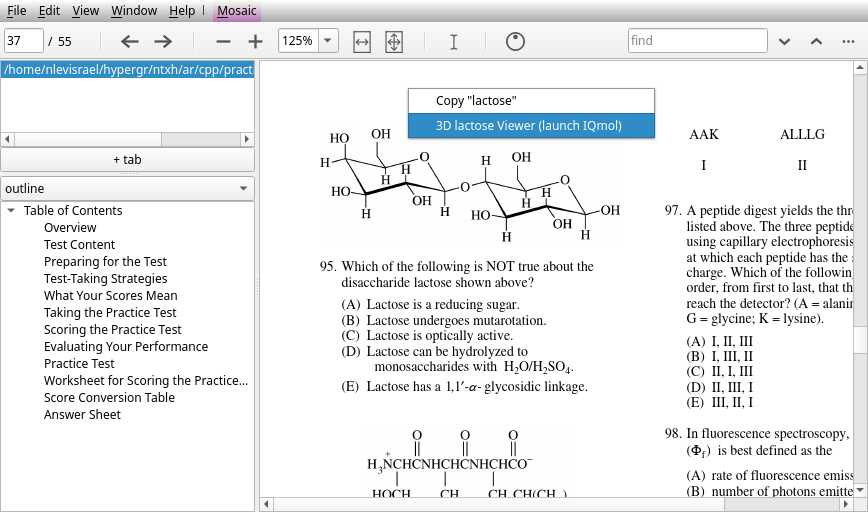
\includegraphics[width=120mm, 
    	trim={0mm 0mm 0mm 0mm},clip]
    	{pics/xl.png}};
    
\end{tikzpicture}   
\end{figure}



\begin{figure}

\caption{Linking PDF Files with Scientific Applications}
\label{fig:il}

\begin{tikzpicture}

\node[inner sep=0pt] (x1) at (0,0)
    {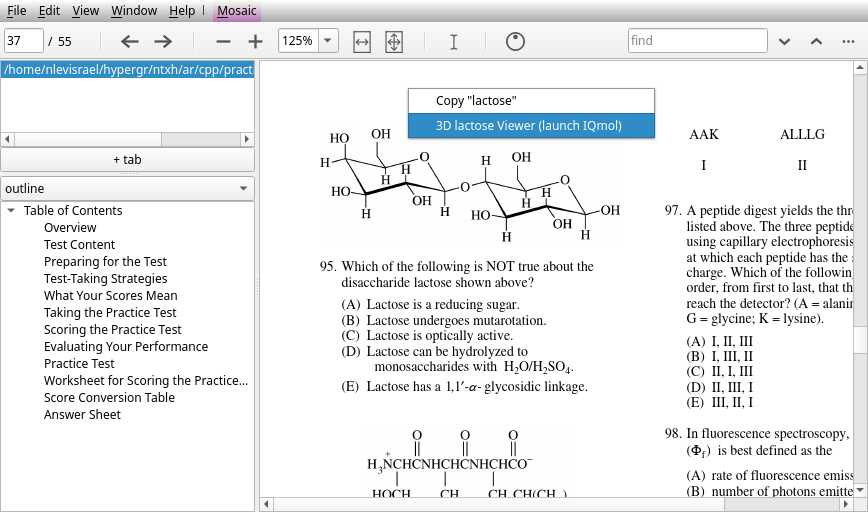
\includegraphics[width=90mm, 
    	trim={0mm 0mm 0mm 0mm},clip]
    	{pics/xl.png}};

\node[inner sep=0pt] (i1) at (10,0)
    {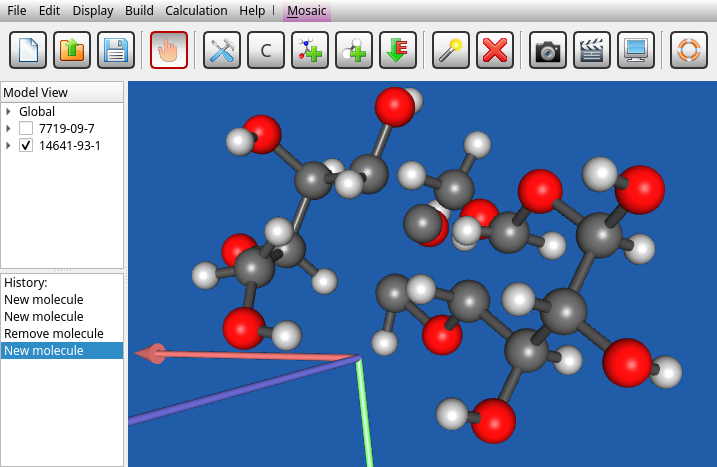
\includegraphics[width=90mm, 
    	trim={0mm 0mm 0mm 0mm},clip]
    	{pics/il.png}};
    
\end{tikzpicture}   
\end{figure}


\p{As a representation of annotation data structures, 
\AXF{} ensures that \SDI{} and viewport data is included 
among annotations wherever this data is available.  
This facilitates the integration between text-mining 
tools and \PDF{} viewer software, which in turn 
enhances reader experience.  As mentioned earlier, every 
annotation can be placed in a semantic context (e.g., 
the text of the surrounding sentence), which provides 
useful reader features such as one-click copying of 
sentences to the clipboard.  Other reader-experience 
enhancements involve multimedia assets.  As a concrete example, 
suppose a paper includes mention of a chemical; that particular 
keyword can accordingly be flagged for annotation.  
As one encoding of the corresponding scientific concept, 
the annotation can include the chemical's Chemical Abstract 
Service Reference Number, via which it is possible to obtain 
Protein Data Bank files to view the molecule in \ThreeD{}.  
Therefore, annotations supply a constellation of data 
--- in this example, concepts may be linked not only to 
identifiers in cheminformatic ontologies, but also to \CAS{} 
reference numbers and thereby to \ThreeD{} graphics files 
--- which facilitate interactive User Experience at the 
application level, not only document classification at the 
corpus level.  Once a chemical compound (mentioned in a 
publication) is linked to a \PDB{} file (or any other 
\ThreeD{} format) the \PDF{} viewer may include 
options to for the reader to connect to software or 
web applications where the corresponding visuals can 
be rendered.  Via \AXF{}, the relevant document-to-software 
connections are asserted not only on the overall document 
level, but on the granular scale of the precise character 
and \PDF{} viewport coordinates where the relevant 
annotation is grounded (Figure~\ref{fig:il} illustrates 
such capabilities in the context of a chemistry publication 
--- specifically, test-preparation materials for the 
Chemistry \GRE{} exam).}

\p{To support this kind of multimedia functionality, 
\AXF{} standardizes a Plugin Framework, dubbed \q{\Mosaic{}}, 
allowing programmers to embed code which can parse and 
respond to \AXF{} annotations in different scientific and 
document-viewer applications.  \lMosaic{} allows different 
applications to inter-operate; in particular, 
\PDF{} viewers can share data with scientific applications 
that can render files in domain-specific formats such as 
\PDB{}.  This application networking protocol is considered 
part of the \AXF{} annotation model, because application-oriented 
information is computationally relevant for many concepts 
encountered in scientific and technical environments.  For instance, 
one aspect of cheminformatic data is that many chemical 
compounds are modeled by \PDB{}, \MOL{}, or \ChemXML{} files, 
which in turn are associated by software applications that 
can load files with those file types.  This inter-application 
networking data then becomes relevant to \PDF{} viewers 
when displaying manuscripts with annotations that suggest 
links to special file types and their applications; the 
viewers can employ this information to launch and/or communicate 
with the corresponding software.  \lAXF{} is designed to 
facilitate implementation of application-networking protocols 
as an operational continuation of processes related to obtaining 
and consuming annotation data.}

\p{The \AXF{} document model, at the manuscript-structure 
level, is paired with a novel \q{Hypergraph Text Encoding 
Protocol} (\HTXN{}) operating at the character-encoding level.  
Within the \HTXN{} protocol, an annotation target is 
a character-index interval in the context of an 
\HTXN{} character stream.  On that basis, 
\HTXN{} treats documents as graphs whose nodes 
are ranges in a character stream, where text can 
be recovered as an operation on one or more nodes 
(e.g., the text of a sentence is derived from a 
pair of nodes representing the sentence's start 
and end).  \lHTXN{} code-points 
are distinguished in terms of their semantic 
role, which may be more granular than their 
visible appearance --- for example, 
a period glyph is assigned different code-points 
depending on whether it marks a sentence-ending 
punctuation, an abbreviation, a decimal point, 
or part of an ellipsis.  Procedures are then implemented to 
represent text in different formats, such as 
\ASCII{}, Unicode, \XML{}, or \LaTeX{}.  In 
contrast to a format such as Web Annotations, 
any particular human-readable text presentation 
(including \ASCII{}) is considered a \textit{derived} 
property of the annotation, not a foundational 
representation.}

\p{\lAXFD{} manuscripts do not need to utilize \HTXN{} 
for character data, but \HTXN{} simplifies certain \AXF{} 
operations, such as identifying sentence boundaries.  
In particular, \HTXN{} provides distinct code-points for 
end-of-sentence punctuation, so that sentence-boundary 
detection reduces to a trivial search for those particular 
code-points.  Proper \HTXN{} encoding requires that authors 
follow certain simple heuristics --- e.g., that end-of-sentence 
periods should be followed by two spaces and/or a newline, 
whereas other uses of a period character should precede at 
most one space.  Aside from the goal of preparing documents 
for text-mining machine-readability, such conventions are 
appropriate even for basic typesetting, because non-punctuation 
characters have distinct kerning rules (this is why 
\LaTeX{} provides a distinct command for non-punctuation glyphs 
that would otherwise be read as punctuation characters).  \lHTXN{} 
hides many of these typesetting details within its character-encoding 
schema, which is useful both for producing professional-caliber 
\LaTeX{} output and for identifying \SDI{} details (such as 
sentence boundaries) which with less rigorously structured 
text would need elaborate text-mining or \NLP{} algorithms.}

\p{Each \AXFD{} document is, in sum, associated with an 
aggregate of character-encoding, annotation, document-structure, 
and \PDF{} viewport information.  The \AXF{} platform uses 
code libraries to pull this information together as a 
runtime object system, so that any application which loads 
an \AXFD{} manuscript can execute queries against the 
corresponding collection of \AXF{} objects (queries such 
as obtaining the sentence text around an annotation, obtaining 
the concave-octagonal viewport coordinates for a sentence,\footnote{
In the general case, sentence coordinates are concave octagons because 
they incorporate the line height of their start and end lines; 
in the general case sentences share start and end lines with other 
sentences, while also including whole lines vertically positioned 
between these extrema.  A sentence octagon roughly corresponds with 
the screen area where a mouse/pointer action should be understood as 
occurring in the context of that sentence from the user's point 
of view --- implying that the user would benefit from context menu 
options pertaining specifically to that sentence, such as 
copy-to-clipboard.} obtaining application-networking 
information for an annotation, 
etc.)  In addition to such runtime data, \AXF{} platforms can 
compile the full suite of information into machine-readable 
files for text and data mining.  These files, collected across a 
corpus of multiple documents, then form the backbone of an 
\AXF{} publication repository, as will be discussed next.}

\section{AXF Publication Repositories}
\p{The \AXF{} platform is designed for hosting collections 
of publications sharing a common academic or technical 
focus.  If \AXF{} is used in the context of a 
general-purpose text and/or data repository, 
the platform is designed to work with collections that 
are organized into separate projects or topics, 
each giving rise to an archive or corpus of publications.  
Insofar as these corpora internally share a common theme 
or focus, they can be associated with their own 
ontologies, code libraries, annotation models, and 
application-networking protocols, based on the sorts 
of applications and data structures commonly used 
in the corresponding scholarly discipline.  
In some cases, publishers may choose to package 
an entire archive of research papers (perhaps along with 
research data) as a single downloadable resource.  
\lAXF{} allows publishers to construct such Research Archives 
following the structure of existing examples such as 
the \ACL{} (Association for Computational Linguistics) 
Anthology or the recent \Cnineteen{} corpus.   This 
latter archive is a useful case-study in both the 
possibilities and limitations of existing 
publication-repository technology.}

\p{\lCnineteen{}, curated by the Allen Institute for 
Artificial Intelligence, was spearheaded by 
a White House initiative to centralize scientific 
research related to \Covid{} (see \cite{CORD}).  The  
collection was formulated with the explicit goal 
of promoting both \textit{text mining} and 
\textit{data mining} solutions 
to advance coronavirus research, so that 
\Cnineteen{} is intended to be used both as a document 
archive for text mining and as a repository for 
finding and obtaining coronavirus data for subsequent 
research.  Although novel research is being 
incorporated into \Cnineteen{}, many of the articles 
reproduced in this corpus are older publications related 
to coronaviruses and to SARS in general, not just to the 
current pandemic.  As a result, the full-text versions 
of these publications were retroactively aggregated 
into a single archive due to the unanticipated emergence 
of a coronavirus crisis, with the full text often obtained 
from \PDF{} files rather than from structured 
representations (such as \JATS{}) explicitly intended 
for text mining.}

\p{This archival methodology results in \Cnineteen{} being 
limited as a \TDM{} framework.  These limitations include 
the following:

\begin{description}
\item[Transcription Errors]  
Transcription errors can easily result from trying to 
read scientific data and notations based on 
\PDF{} files --- or on full-text representations using 
relatively unstructured formats such as \XOCS{} 
(the response-encoding format for the ScienceDirect 
\API{}).  Transcription errors cause the machine-readable 
text archive to misrepresent the structure 
and content of documents.  For instance, 
there are cases in \Cnineteen{} 
of scientific notation and terminology 
being improperly encoded.  As a concrete example, \colorq{2{\textquotesingle}-C-ethynyl} is encoded incorrectly in one \Cnineteen{} file 
as \makebox{\colorq{2 0 -C-ethynyl}} (see \cite{Eyer} for 
the human-readable publication where this error is 
observed; the corresponding index in the corpus is \textcolor{blGreen!45!black}{9555f44156bc5f2c6ac191dda2fb651501a7bd7b.json}).  
To help address these sorts of errors --- 
which could stymie text searches 
against the \Cnineteen{} corpus --- 
it is obviously preferable to archive structured, 
machine-readable versions of publications, using 
a platform such as \AXF{}.  
    
\item[Converting Between Data Formats]
Although the \Cnineteen{} corpus is published 
as \JSON{} files, many text-mining tools such 
as those reviewed in \cite{NeusteinText} recognize 
inputs or produce outputs in alternative formats, 
such as \XML{}, \BioC{}, \CoNLL{} (Conference on Natural 
Language Learning), or \JSON{} trees with 
different schema than \Cnineteen{}.  For this 
reason, rather than providing data with one single 
representational format, it is better to 
encode the data along with code libraries that can 
express the data in different formats as needed 
for different \TDM{} ecosystems.

\item[Inconsistent Annotations]  
The structure of \Cnineteen{} allows text segments to 
be defined via a combination of \JSON{} file names, 
paragraph ids, and character indices.  This indexing 
schema is used for representing certain internal 
details of individual articles, such as citations, 
but is not explicitly defined as an annotation 
target structure for standoff annotations against 
the archive as a whole.  This problem could 
also be rectified with code libraries that map 
index targets to file handles and character pointers. 

\item[Limited Support for Research Data-Mining]  Even though 
many papers in \Cnineteen{} are paired with 
published data sets, there is currently no tool for 
locating  research \textit{data} 
through \Cnineteen{}. 
For example, the collection of manuscripts available 
through the Springer Nature portal linked 
from \Cnineteen{} includes over 30 \Covid{} data sets,
but researchers can only discover that these data 
sets exist by looking for a \q{supplemental materials} or 
a \q{data availability} addendum near the end of each article.
These Springer Nature data sets encompass a wide array of file types 
and formats, including \FASTA{} (which stands for Fast-All, 
a genomics format), \SRA{} (Sequence Read Archive, for 
\DNA{} sequencing), \PDB{} (Protein Data Bank,  
representing the \ThreeD{} geometry of protein 
molecules), \MAP{} (Electron Microscopy Map), \EPS{} 
(Embedded Postscript), \CSV{} (comma-separated values), 
and tables represented in Microsoft Word 
and Excel formats.  To make this data more 
readily accessible in the context of \Cnineteen{}, it 
would be appropriate to (1) maintain an index of 
data sets linked to \Cnineteen{} articles 
and (2) merge these resources into a common representation 
(such as \XML{}) wherever possible.  This research-data 
curation can then be treated as a supplement to 
text-mining operations.  In particular, queries 
against the full-text publications could be evaluated 
\textit{also} as queries against the relevant set 
collection of research data sets.    

\item[Wrappers for Network Requests]  Scientific 
use of \Cnineteen{} will often require communicating 
with remote servers.  For example, genomics 
information in the \Covid{} data sets (such as 
those mentioned above that are available through 
Springer Nature) is generally 
provided in the form of accession numbers which 
are used to query online genomics services.  
Similarly, text mining algorithms often 
rely on dedicated servers to perform 
Natural Language Processing; these services 
might take requests in \BioC{} format and respond 
with \CoNLL{} data.  As another case study epidemiological 
studies of \Covid{} may need to access \API{}s or data 
sets such as the John Hopkins University \q{dashboard} 
(see \href{https://coronavirus.jhu.edu/map.html}{https://coronavirus.jhu.edu/map.html}, which is paired with a \GIT{} archive 
updated almost daily).  To reduce the amount 
of \q{biolerplate code} which developers need 
for these networking requirements, an archive's 
text-mining code could provide a unified framework with which 
to construct web-\API{} queries, 
one that could be used across 
disparate scientific disciplines 
(genomics, \NLP{}, epidemiology, and so forth). 
\end{description}}

\p{Many of these limitations observed in \Cnineteen{} 
reflect the fact that this corpus was prepared 
as \q{raw (text) data} without any supporting code.  
Recent initiatives, such as the Research Object 
protocol (see \cite{KhalidBelhajjame}) 
and \FAIR{} (\q{Findable, Accessible, 
Interoperable, Reusable}; see \cite{TrifanOliveira}) 
encourage authors to publish code and data together, 
so that the computing environment needed to process 
published data is provided within the data set itself.  
This Research Object model is usually defined in 
the context of a single publication, but the paradigm 
applies equally well to corpora encompassing many 
single articles.  That is, \AXF{} is structured so 
that Research Archives can be designed as higher-scale 
Research Objests, wherein the document collection is bundled 
with supporting code and an overall computing and 
software-development environment.  Such archive-specific 
\SDK{}s would include \AXF{}-specific code as well 
as libraries or applications often utilized in 
the academic disciplines relevant to the archival 
subject areas.  The \AXF{} platform especially 
promotes the design of domain-specific \SDK{} 
which are \textit{standalone} 
and \textit{self-contained}, with minimal external 
dependencies.  As much as possible, users should 
not have to install external software to utilize 
data provided along with an \AXF{} repository; 
instead, the needed data-management tools should be 
provided in source-code form within the archive itself.}

\p{Each \AXF{} repository, then, should 
bundle numerous applications used for database 
storage, data visualization, and scripting.  
The goal of this application package would be to 
provide researchers with a self-contained computing 
platform optimized for scientific research 
and findings related to the archived publications.  
Archival \SDK{}s should try 
to eliminate almost all scenarios where 
programmers would need to perform a \q{system 
install}; for the most part, the entire 
computing platform (including scripting 
and database capabilities) should be compiled 
from source \q{out-of-the-box}.  While the 
actual libraries and applications bundled with 
an archive would depend on its topical 
focus, the following is an example of components 
that would be appropriate in many different \SDK{}: 

\begin{itemize}[itemsep=-1pt]

\item \XPDF{}: A \PDF{} viewer for reading full-text articles 
(augmented with \Cnineteen{} features, such as integration 
with biomedical ontologies);

\item \Qt{}: The \Qt{} library is a cross-platform 
Application-Development framework and 
\GUI{} toolkit commonly used for scientific applications 
(\XPDF{} is one example of a \Qt{}-based document 
viewer).  Almost any data set can be accompanied 
with \Qt{} code for data visualization, so that readers 
would not have to install additional software.  For its 
part, \Qt{} can be freely obtained and, once 
downloaded, resides wholly in its own folder 
(there is no install step which modifies the 
user's system); as such, \Qt{} along with individual 
archive \SDK{}s function as standalone packages, 
although optimally the \SDK{}s would be updated along with 
new \Qt{} versions.  
  
\item AngelScript: An embeddable scripting engine 
that could be used for analytic processing 
of data generated by text and data mining operations 
on \Cnineteen{} (see \cite{AS});

\item WhiteDB: A persistent database 
engine that supports both relational 
and \NoSQL{}-style architectures 
(see \cite{EnarReilent});

\item MeshLab: A general-purpose \ThreeD{} graphics 
viewer;

\item LaTeXML: a \LaTeX{}-to-\XML{} converter;

\item PositLib: a library for use in high-precision computations based on the \q{Universal Number} format, 
which is more accurate than traditional floating-point 
encoding in some scientific contexts 
(see \cite{JohnGustafson}). 
\end{itemize}

To this list one might add components specific to various 
scientific fields: \IQmol{} for chemistry and molecular 
biology, for example, or open-source libraries such 
as EpiFire or Simpact (for Epidemiology), \UDpipe{} (for 
\CoNLL{}), and so forth.  Here again the priority 
would be for self-contained components with few 
external dependencies --- particularly libraries 
programmed in \C{} or \Cpp{}, which are the 
languages best positioned to be a common denominator 
across diverse research projects (of course, many 
scientific \Cpp{} libraries have wrappers for 
languages like \R{} or Python that researchers may be 
more comfortable using).  
In general, Research Archive code should be 
(1) \textit{self-contained} (with few or no external 
dependencies); (2) \textit{transparent} (meaning that 
all computing operations should be implemented by 
source code within the bundle that can be examined 
as code files and within a debugging session); 
and (3) interactive (meaning that the bundle does not 
only include raw data but also software to interactively 
view and manipulate this data).  Research Archives which 
embrace these priorities attempt to provide data visualization, 
persistence, and analysis through \GUI{}, database, and 
scripting engines that can be embedded as source 
code in the archive itself. }
  
\p{It is worth noting that a data-mining platform requires 
\textit{machine-readable} open-access research data
(which is a more stringent requirement than simply 
pairing publications with data that can only 
be understood by domain-specific 
software).  For example, radiological imaging can be a source 
of \Covid{} data insofar as patterns of lung 
scarring, such as \q{ground-glass opacity,} are a leading 
indicator of the disease.  Consequently, diagnostic 
images of \Covid{} patients are a relevant kind of 
content for inclusion in a \Covid{} data set 
(see \cite{Shi} as a case-study).  However, 
diagnostic images are not in themselves 
\q{machine readable.}  When medical imaging is 
used in a quantitative context (e.g., applying 
Machine Learning for diagnostic pathology), it is necessary 
to perform Image Analysis to convert the raw data 
--- in this case, radiological graphics --- into 
quantitative aggregates.  For instance, by using image 
segmentation to demarcate geometric boundaries one 
is able to define diagnostically relevant features (such 
as opacity) represented as a scalar field over the segments.  
In short, even after research data is openly published, 
it may be necessary to perform 
additional analysis on the data for it to be 
a full-fledged component of a 
machine-readable information space.\footnote{%
\raisebox{-10pt}{\hspace{3pt}\parbox{.9\textwidth}{This does not mean that diagnostic images (or 
other graphical data) should not be placed in a 
data set; only that computational reuse of such 
data will usually involve certain numeric 
processing, such as image segmentation.  
Insofar as this subsequent analysis is performed, 
the resulting data should wherever possible 
be added to the underlying image data as a 
supplement to the data set.}}}  To 
deal with this sort of situation, \AXF{} equips 
\SDK{}s with a \textit{procedural 
data-modeling vocabulary} that would both identify the 
interrelationships between data representations 
and define the workflows needed to 
convert research data into machine-readable data sets.} 

\p{Another concern in developing an integrated Research Arcive
data collection is that of indexing documents and research findings  
for both text mining \textit{and} data mining.  
In particular, \AXF{} introduces a 
system of \textit{microcitations} that apply 
to portions of manuscripts \textit{as well as} data sets.  
In the publishing context, a microcitation is defined as a 
reference to a partially isolated fragment of a larger 
document, such as a table or figure illustration, or a 
sentence or paragraph defining a technical term, 
or (in mathematics) the statement/proof of a definition, axiom, 
or theorem.  In data publishing, \q{data citations} are 
unique references to data sets in their entirety or to 
their smaller parts.  A data microcitation is then a 
fine-grained reference into a data set.  For example, 
a data microcitation can consist of one 
column in a spreadsheet, 
one statistical parameter in a quantitative analysis, 
or \q{the precise data records actually used in a study} 
(in the words adopted by the Federation of Earth Science Information Partners to define microcitations; 
see \cite{ESIP}).  As a concrete example, 
a concept such as \q{expiratory flow} appears in \Cnineteen{} 
both as a table column in research data and as a medical concept 
discussed in research papers; a unified microcitation framework 
should therefore map \textit{\color{drp}{expiratory flow}} as a keyphrase 
to both textual locations and data set parameters.  
Similarly, a concept such as 
\textit{\color{drp}{2{\textquotesingle}-C-ethynyl}} (mentioned earlier, in the context of transcription errors) 
should be identified both as a phrase in 
article texts and as a molecular component 
present within compounds whose scientific 
properties are investigated through \Cnineteen{} 
research data.  In so doing, a search for this 
concept would then trigger both publication and 
data-set matches at the same time.}

\p{Further discussion on data microcitations depends on 
how data sets are structured, which is addressed in the next section.}


\section{Research Objects and Data Microcitations}
\p{The design of \AXF{} assumes that many Research Archives, 
comprising of multiple publications sharing an academic 
focus, will also include open-access research data.  
The primary motivation for publishing 
research data is to ensure transparency and 
reusability: open-access data allows readers to verify 
that scientific/technical claims are warrented, 
and/or to reuse or incorporate existing data into 
new research.  Open-access data has other purposes 
as well: data sets, for example, can serve 
as pedagogic tools helping readers understand 
publications' concepts experimentally and 
interactively (a good example is \cite{AlexandruTelea}, 
which pairs data sets with most chapters to 
illustrate principles in data visualization).  
Moreover, the theory informing how data sets are 
organized can serve as a technical exposition 
of research principles and methodology.  For all 
of these reasons, open-access data is an 
increasingly important part of the publishing 
ecosystem.  This means 
that well-curated archives will often need to 
prepare data sets for data 
mining, alongside the preparation of text materials for 
text mining.  }

\p{In contrast to text mining, however, it is not feasible, 
in the general case, to 
assign one single format (like \AXFD{} or \JATS{}) for all 
data sets published within an archive.  Precisely how data 
sets can be annotated depends on the data models, programming 
languages, and analytic methodologies which they utilize.  
Because this variability prohibits a single data-annotation 
protocol from being required, \AXF{} adopts a strategy of 
defining a rigorous protocol for \Cpp{} code bases, which 
can then be emulated by other languages.}


\begin{figure}

\caption{Data Microcitations via Tabular Columns}
\label{fig:oxy}

\begin{tikzpicture}

\node[inner sep=0pt] (x1) at (0,0)
    {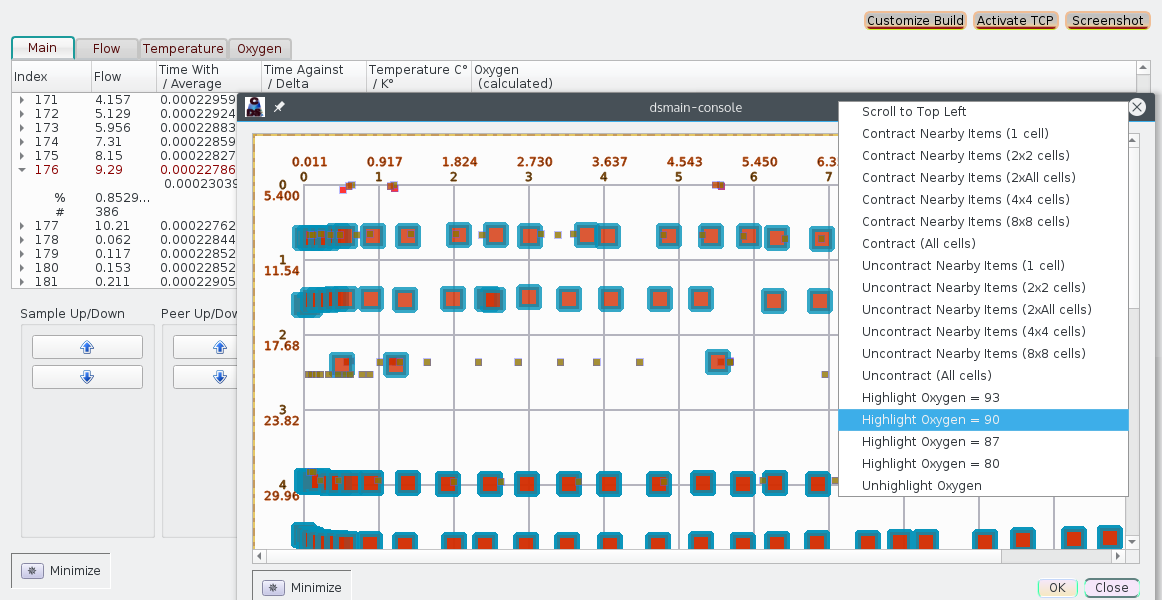
\includegraphics[width=180mm, 
    	trim={0mm 0mm 0mm 0mm},clip]
    	{pics/oxy.png}};
    
\end{tikzpicture}   
\end{figure}


\p{As outlined above, data citations refer to parts within a 
data set --- such as individual data records, but also larger-scale 
aggregates such as table columns or statistical parameters.  
The complication when defining data citations is that a 
concept such as a table column, although it may have an 
obvious technical status as a discrete conceptual unit from 
the point of view of scientists curating, studying or reusing 
a data set, does not necessarily correspond to a single 
coding entity that could be isolated as an annotation 
target.  It is therefore the responsibility of 
\textit{code base annotations} to provide annotations for 
computational units --- such as data types, procedures, and 
\GUI{} components --- that have an annotatable \textit{conceptual} 
status relative to the data set on which the code operates.  
Often this will involve mapping one concept to 
several computational units (for instance, several 
procedure implementations).}

\p{For a concrete example of these points concerning 
data citations, consider the data set pictured 
in Figure~\ref{fig:oxy}, representing cyber-physical measurements 
used to calculate oxygenated airflow.  The data-set 
application displays tabular data via a tree widget 
(which functions as a generalized, multi-scale spreadsheet 
table), with tabular columns expressing quantities such 
as air flow and oxygen levels in several formats (raw 
measures as well as sample rankings and min-max 
percentages).  Conceptually, these columns have distinct 
methodological roles and therefore can be microcited; 
indeed, the application links the columns to article 
text where the corresponding concepts are presented 
(see Figure~\ref{fig:about}).  However, the implementation does not introduce 
a distinct \Cpp{} object uniquely designating individual 
columns.  Instead, the individual columns can be annotated 
in terms of \Cpp{} methods providing column-specific 
functionality.  In the current example, these methods 
primarily take the form of features linked to context-menu 
actions (copying column data to the clipboard, sorting data 
by one column, etc.).  In general, rather than a rigid 
protocol for data-set annotations, \AXF{} proposes 
heuristic guidelines for how best to map programming 
constructs to scientifically salient data-set concepts.}


\begin{figure}

\caption{Linking Dataset Applications to Publications}
\label{fig:about}

\begin{tikzpicture}

\node[inner sep=0pt] (x1) at (0,0)
    {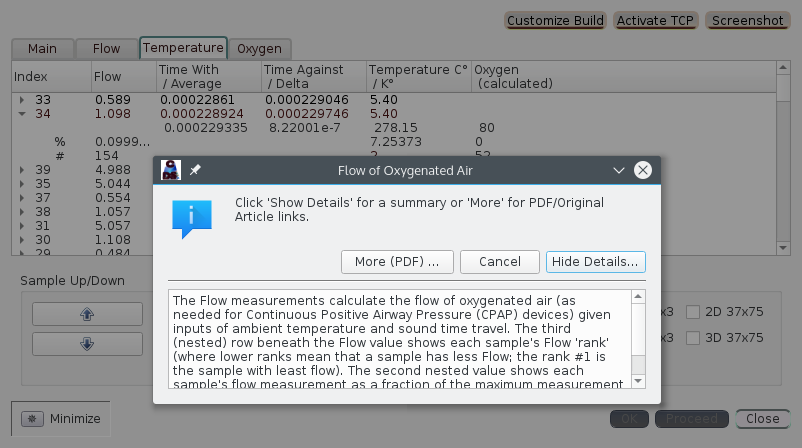
\includegraphics[width=180mm, 
    	trim={0mm 0mm 0mm 0mm},clip]
    	{pics/about.png}};

\end{tikzpicture}    
\end{figure}


\p{Defining an annotation schema for data sets can potentially 
be an organic outgrowth of software-development methodology, 
such as implementing unit tests.  This point is illustrated in 
Figure~\ref{fig:testing}, which shows a \GUI{}-based testing environment for 
the data set depicted in Figures~\ref{fig:about} and \ref{fig:oxy}.  For this data set, 
the context menu actions providing column-specific functionality 
are also discrete capabilities which can be covered by 
unit tests, so the set of procedures mapped to the citeable 
concept correspond with a set of unit-test requirements.  
In this data set, these procedures are also exposed to 
scripting engines via the \Qt{} meta-object system.  In general, 
there is often a structural correlation between 
scripting, unit testing, and microcitation, so that 
an applications' scripting and testing protocol can serve 
as the basis for annotation schema.  For data sets which use 
in-memory or persistent databases, evaluable queries against 
these databases provide an additional grounding for annotations.  
In general, data-annotation should be designed on the 
basis of a dataset applications' scripting, testing, and/or 
query-evaluation code.  However, this is only a heuristic 
guideline, and \AXF{} does not presuppose any data-annotation 
scheme \textit{a priori}.}

    \begin{frame}{\ft{Testing}}

        \begin{annotatedFigure}{0pt}{0pt}
            {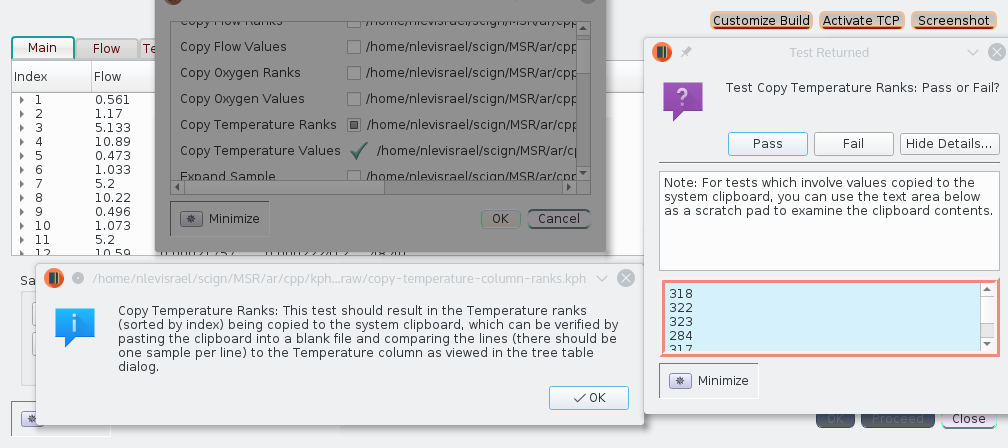
\includegraphics[scale=1]{texs/testing.png}}
            
  \node [text width=20cm,align=justify,fill=logoCyan!20, draw=logoBlue, 
  draw opacity=0.5,line width=1mm, fill opacity=0.9]
   at (0.38,0.93){\textbf{Dataset Creator includes a sophisticated 
   framework for building and running test suites to 
   ensure that raw data is processed correctly and that 
   User Interface components work properly on different 
   Operating System platforms.  This includes 
   a separate testing application that sends instructions 
   to the main Dataset Application via TCP (\circled{1}).}};

  \annotatedFigureBox{0.81,0.93}{0.903,0.982}{1}{0.903,0.935}%
  
  
   \node [text width=4cm,align=justify,fill=logoCyan!20, draw=logoBlue, 
   draw opacity=0.5,line width=1mm, fill opacity=0.9]
    at (0.08,0.64){\textbf{The testing application has several 
    features to facilitate running tests, including 
    options to repeat tests, mark success or failure (\circled{2}), and 
    examine the system clipboard (\circled{3}).}};
 
  \annotatedFigureBox{0.17,0.63}{0.37,0.685}{2}{0.37,0.63}
   \annotatedFigureBox{0.651,0.113}{0.995,0.86}{3}{0.892,0.86}% 

   \node [text width=11cm,align=justify,fill=logoCyan!20, draw=logoBlue, 
   draw opacity=0.5,line width=1mm, fill opacity=0.9]
    at (0.26,0.09){\textbf{Testers can 
    also read a description of each test (\circled{4}),  
    and view the scripts used to ceate them.}};
 
  \annotatedFigureBox{0.05,0.16}{0.62,0.325}{4}{0.62,0.19}
  
      %      \annotatedFigureBox{0.222,0.284}{0.3743,0.4934}{B}{0.3743,0.4934}%tr
      %      \annotatedFigureBox{0.555,0.784}{0.6815,0.874}{C}{0.555,0.784}%bl
      %      \annotatedFigureBox{0.557,0.322}{0.8985,0.5269}{D}{0.8985,0.5269}%tr
  
        \end{annotatedFigure}

    \end{frame}




%a file in formats such as \CoNLL{} or \PMML{} 
%(Predictive Model Markup Language).}
%\p{Operationally, \AXF{} is modeled most 
%directly on the BeCAS \API{} \cite{TiagoNunes} 
%and the Linguistic Annotation Framework (\LAF{}).\footnote{%
%such as \PMML{}, \ARFF{} (Attribute-Relation File Format), 
%interface based on BeCAS.  Moreover, 

\section{Conclusion}
\p{\AXF{} uses a two-tier node structure similar to 
\LAF{}; at one level is an extensible text-encoding 
methodology (disussed in the next paragraph), 
while a higher level defines annotations in terms 
of directed hypergraphs.  Programmatically, 
\AXF{} aims in the canonical case for a level of 
detail that is intermediate between linked-data-oriented 
projects like Web Annotations (which tend to focus 
mostly on isolatable semantic resources such 
as citations and named entities) and \NLP{}-oriented 
paradigms such as \LAF{}.  That is, \AXF{} does not 
natively serialize fine-grained \NLP{} data at the 
level of individual words (the kind of data asserting 
semantic and morphosyntactic details: lemmatization, Part of Speech, 
dependency relations, and so forth), although it does support 
queries which return sentences as (unparsed) word-sequences.  
On the other hand, \AXF{} offers \text{some} granular information about 
small-scale linguistic units, such as the 
role of non-alphanumeric characters, or 
\PDF{} coordinates of sentence start and end points.  
In short, \AXF{} occupies a unique space in the 
landscape of annotation tools at the intersection 
of application-development, \NLP{}, and document-preparation 
requirements.}

\vspace{-.75em}
%\noindent\lun{ETS\textsc{pf} for Scientific and Technical Applications}

\setlength{\bsep}{-6pt}
%\setlength{\parskip}{0pt}
%\setlength{\itemsep}{-2pt}

\makeatletter
    \clubpenalty10000
    \@clubpenalty \clubpenalty
    \widowpenalty10000
\makeatother

\begin{thebibliography}{99}
\vspace{.5em}
{\fontsize{10}{11}\selectfont

\bibitem{RaubalAdams}
Benjamin Adams and Martin Raubal, 
\q{A Metric Conceptual Space Algebra}.
\biburl{https://pdfs.semanticscholar.org/521a/cbab9658df27acd9f40bba2b9445f75d681c.pdf}

\bibitem{RaubalAdamsCSML}
Benjamin Adams and Martin Raubal, 
\q{Conceptual Space Markup Language (CSML): Towards the Cognitive Semantic Web}.
\biburl{http://idwebhost-202-147.ethz.ch/Publications/RefConferences/ICSC_2009_AdamsRaubal_Camera-FINAL.pdf}

\bibitem{KhalidBelhajjame}{%
	Khalid Belhajjame, \textit{et. al.},
	\q{Workflow-centric research objects:  First class citizens in scholarly discourse}.	\biburl{https://pages.semanticscholar.org/coronavirus-research}}

\bibitem{InteractingConceptualSpaces}
Joe Bolt, \i{et. al.}, 
\cq{Interacting Conceptual Spaces I:
Grammatical Composition of Concepts}.
\biburl{https://arxiv.org/pdf/1703.08314.pdf}

\bibitem{CORD}{%
	\q{COVID-19 Open Research Dataset (CORD-19)}. 2020. Version 2020-03-13. Retrieved from https://pages.semanticscholar.org/coronavirus-research. Accessed 2020-03-20. doi:10.5281/zenodo.3715506
	\biburl{https://pages.semanticscholar.org/coronavirus-research}}
\bibitem{Eyer}{%
	Lud\"ek Eyer, \textit{et. al.},
	\q{Nucleoside analogs as a rich source of antiviral agents active against arthropod-borne flaviviruses}.
	\biburl{https://www.ncbi.nlm.nih.gov/pmc/articles/PMC5890575/}}

\bibitem{Zenker}
Peter G\"ardenfors and Frank Zenker,  
\cq{Theory Change as Dimensional Change: Conceptual Spaces 
	Applied to the Dynamics of Empirical Theories}.
\intitle{Synthese 190(6)}, pp. 1039-1058, 2013.  
\biburl{http://lup.lub.lu.se/record/1775234}

\bibitem{JohnGustafson}{%
	John Gustafson,
	\q{Beating Floating Point at its Own Game: Posit Arithmetic}, 
	\biburl{http://www.johngustafson.net/pdfs/BeatingFloatingPoint.pdf}}

\bibitem{IdeSuderman}{%
	Nancy Ide and Keith Suderman,
	\q{GrAF: A Graph-based Format for Linguistic Annotations}, 
	\biburl{https://www.cs.vassar.edu/~ide/papers/LAW.pdf}}

\bibitem{AS}{%
	Andreas J\"onsson,
	\q{AngelCode Scripting Library}, 
	\biburl{www.AngelCode.com/AngelScript/}}

\bibitem{NeusteinText}{%
	Amy Neustein, \textit{et. al.},
	\q{Application of Text Mining to Biomedical Knowledge Extraction: Analyzing Clinical Narratives and Medical Literature}, 
	\biburl{https://www.researchgate.net/publication/262372604_Application_of_Text_Mining_to_Biomedical_Knowledge_Extraction_Analyzing_Clinical_Narratives_and_Medical_Literature}}

\bibitem{TiagoNunes}{%
	Tiago Nunes, \textit{et. al.},
	\q{BeCAS: biomedical
concept recognition services and visualization}.
	\biburl{https://www.ncbi.nlm.nih.gov/pubmed/23736528}}

\bibitem{ESIP}{%
Mark A. Parsons and Ruth Duerr,
\q{Data Identifiers, Versioning, and Micro-citation}, 
\biburl{https://www.thelancet.com/action/showPdf?pii=S1473-3099\%2820\%2930086-4}}

\bibitem{EnarReilent}{%
	Enar Reilent,
	\q{Whiteboard Architecture for the Multi-agent Sensor Systems}, 
	\biburl{https://www.thelancet.com/action/showPdf?pii=S1473-3099\%2820\%2930086-4}}

\bibitem{Shi}{%
	Heshui Shi, \textit{et. al.},
	\q{Radiological findings from 81 patients with COVID-19 
		pneumonia in Wuhan, China: a descriptive study}.
	\biburl{https://www.thelancet.com/action/showPdf?pii=S1473-3099\%2820\%2930086-4}}

\bibitem{DietrichRebholzSchuhman}{%
	Dietrich Rebholz-Schuhman, \textit{et. al.},
	\q{IeXML: towards an annotation framework for biomedical semantic types enabling interoperability of text processing modules}.
	\biburl{https://www.semanticscholar.org/paper/IeXML\%3A-towards-an-annotation-framework-for-semantic-Rebholz-Schuhmann-Kirsch/1d72a56b6576117c62f388a5f2193965e4c7e293}}

\bibitem{CJRupp}{%
	C. J. Rupp, \textit{et. al.},
	\q{Flexible Interfaces in the Application of Language Technology to an eScience Corpus}.
	\biburl{https://www.cl.cam.ac.uk/~sht25/papers/Rupp_et_al.pdf}}

\bibitem{AlexandruTelea}{%
	Alexandru Telea,
	\q{Data Visualization --- Principles and Practice}.
	\biburl{https://www.semanticscholar.org/paper/Data-visualization-principles-and-practice-Telea/c853f4b8aee67cd749e03b3a4413769792222776}}


\bibitem{TrifanOliveira}{%
	Alina Trifan and Jos\'e Lu\'\i{}s Oliveira,
	\q{FAIRness in Biomedical Data Discovery}.
	\biburl{https://www.researchgate.net/publication/331775411_FAIRness_in_Biomedical_Data_Discovery}}

\bibitem{EricWinsberg}{%
	Eric Winsberg, \textit{Science in the Age of Computer Simulation}.
	\biburl{https://www.press.uchicago.edu/ucp/books/book/chicago/S/bo9003670.html}}

}
\end{thebibliography}

\end{document}


